% !TEX root = ../main.tex
\chapter{Resultados y análisis}\label{cap:evaluacion}

Este capítulo presenta el análisis cuantitativo y cualitativo de los resultados obtenidos en cada caso de uso, discute las diferencias de rendimiento entre algoritmos cuánticos y clásicos a la luz del estado del arte, y evalúa las implicaciones prácticas para su aplicación en el contexto operativo de SKG Tecnología. Para cada caso se identifican explícitamente las condiciones bajo las que se observa ventaja cuántica, las limitaciones que explican los resultados negativos, y las perspectivas de mejora a medida que el hardware cuántico avance.

% =====================================================================
\section{Caso de uso 1: Clasificación supervisada}
% =====================================================================

\subsection{Dataset cuántico-nativo: ventaja cuántica demostrada}

Los resultados sobre el dataset con estructura cuántica explícita constituyen la demostración empírica más sólida del estudio. El QSVM alcanzó una exactitud del \textbf{91.7\%}, frente al 53.3\% del mejor clasificador clásico (SVM polinomial de grado 3; SVM-RBF: 46.7\%, Gradient Boosting: 51.7\%, SVM lineal: 45.0\%), lo que supone una \textbf{ventaja de +38.3 puntos porcentuales (pp)}. Este resultado es el esperado por construcción, y coherente con la idea de \cite{liu2021} y \cite{huang2021} de que la ventaja exige un kernel alineado con las etiquetas: cuando estas se definen mediante una función cuántica, el kernel cuántico las aprende con alta precisión mientras que los clasificadores clásicos probados (RBF, polinomial, lineal y Gradient Boosting) quedan cerca del azar.

El análisis de escalabilidad (Tabla~\ref{tab:escala_clasificacion}) muestra que esta ventaja no depende de un tamaño de muestra particular: es positiva en todo el rango $n \in [30, 180]$ evaluado, con una ventaja media de \textbf{+40.9 pp} y una máxima de \textbf{+48.9 pp} para $n=50$.

\begin{table}[h]
\centering
\begin{tabular}{ccccc}
\hline
\textbf{$n$ train} & \textbf{QSVM (\%)} & \textbf{Mejor clásico (\%)} & \textbf{Ventaja (pp)} \\
\hline
30  & 88.9 & 46.7 (SVM-RBF) & +42.2 \\
50  & 91.1 & 42.2 (SVM-RBF) & +48.9 \\
80  & 85.6 & 48.9 (SVM-RBF) & +36.7 \\
100 & 85.6 & 47.8 (SVM-RBF) & +37.8 \\
140 & 88.9 & 44.4 (SVM-RBF) & +44.4 \\
180 & 91.1 & 55.6 (SVM-RBF) & +35.6 \\
\hline
\textbf{Media} & \textbf{88.5} & \textbf{47.6} & \textbf{+40.9} \\
\hline
\end{tabular}
\caption{Escalabilidad de la ventaja cuántica en clasificación (dataset cuántico-nativo, ZZFeatureMap 2 qubits).}
\label{tab:escala_clasificacion}
\end{table}

\begin{figure}[ht]
\centering
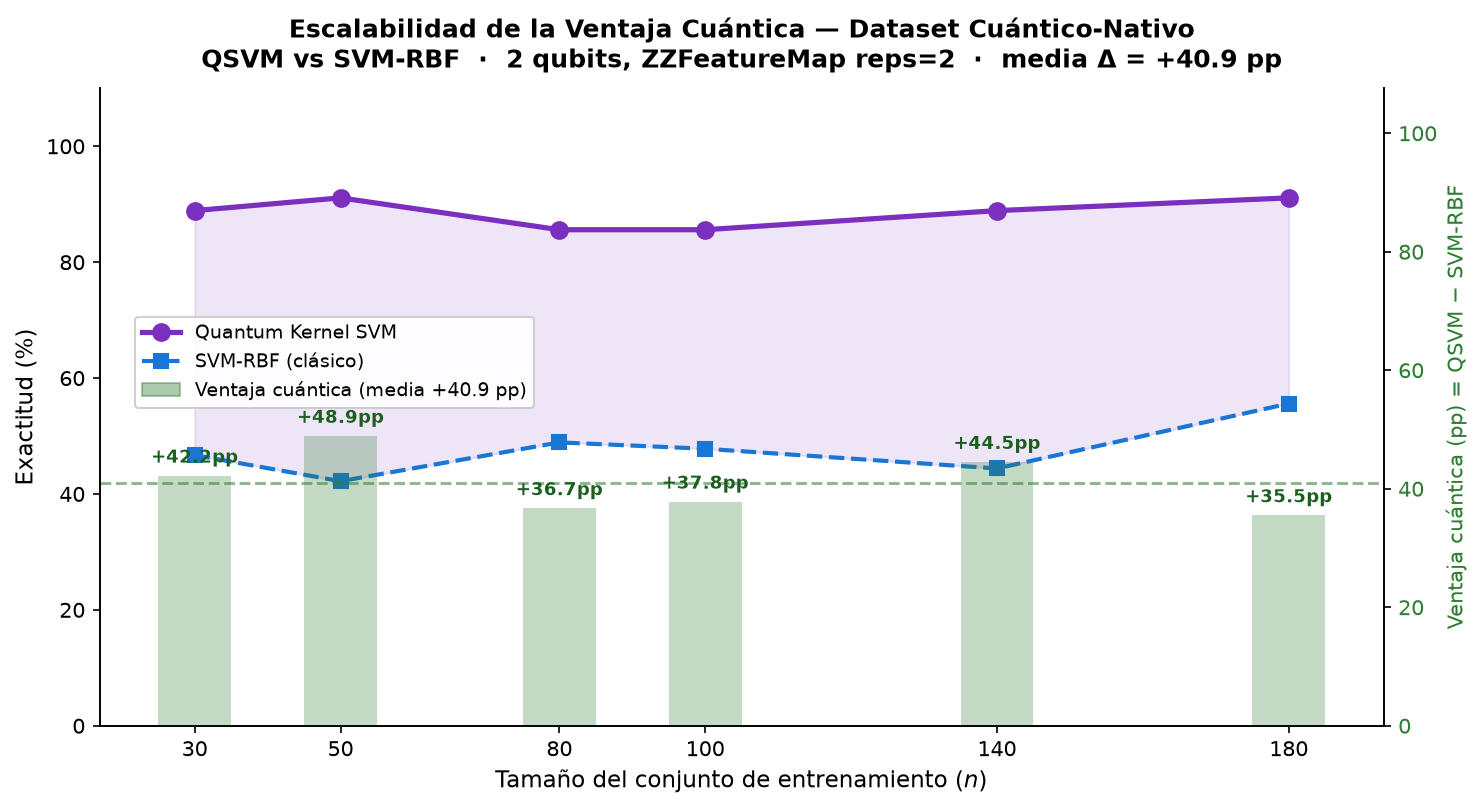
\includegraphics[width=0.92\textwidth]{../POCs/data/output/figures/01_escalabilidad_ventaja_clasificacion.png}
\caption{Escalabilidad de QSVM vs.\ SVM-RBF en el dataset cuántico-nativo según el tamaño del conjunto de entrenamiento ($n \in [30, 180]$; salida del Notebook~01). Izquierda: exactitud en test de ambos modelos. Derecha: ventaja del QSVM en puntos porcentuales, positiva en todos los tamaños evaluados (media $+40.9$~pp). Cada punto es una única partición, por lo que las diferencias entre tamaños no son estadísticamente concluyentes; los datasets reales (SKG, Telco) no se evaluaron en esta curva.}
\label{fig:escala_clasificacion}
\end{figure}

El mecanismo que explica esta ventaja es la \textbf{alineación} entre el feature map y el generador de etiquetas: en este experimento ambas son el mismo \texttt{ZZFeatureMap} (mapa empíricamente validado en el TFM), de modo que el kernel minimiza el riesgo empírico en el \textbf{espacio de representación} correcto ---el espacio de Hilbert $\mathcal{H}$ inducido por $\phi\colon\mathbb{R}^2\rightarrow\mathcal{H}$---. La lección no es ``ZZ gana'', sino ``el mapa alineado gana''. Los clasificadores clásicos operan en $\mathbb{R}^2$ y no acceden a ese espacio de Hilbert sin coste exponencial.

\paragraph{Limitaciones que condicionan la interpretación.}
\begin{itemize}
  \item El dataset es artificial: está diseñado a medida para el kernel cuántico. La ventaja observada es una cota superior del rendimiento cuántico en condiciones ideales.
  \item La simulación exacta sin ruido es optimista respecto al hardware NISQ real; la decoherencia reduciría la fidelidad del kernel y, por tanto, la ventaja.
  \item El coste cuadrático $O(n^2)$ del kernel limita la escala evaluable; en producción, $n > 1{,}000$ sería computacionalmente inviable en simulación.
\end{itemize}

\begin{figure}[ht]
\centering
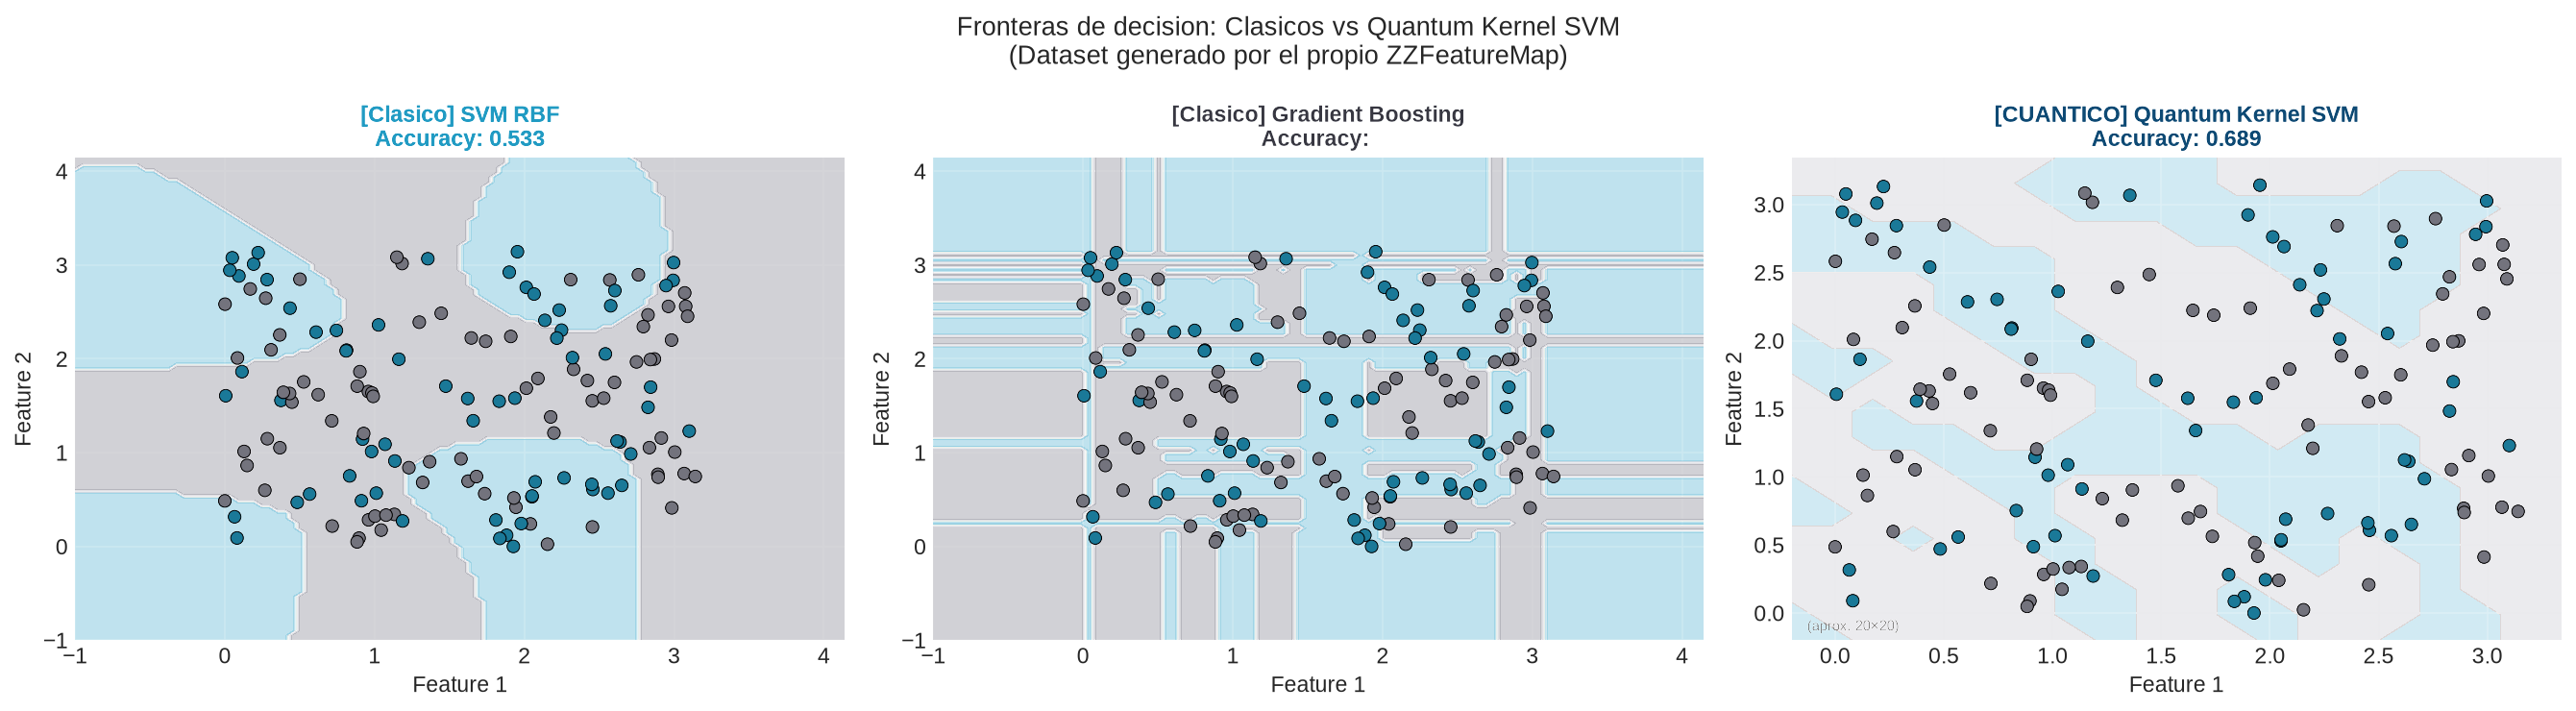
\includegraphics[width=0.95\textwidth]{../POCs/data/output/figures/06_quantum_kernel_boundaries.png}
\caption{Fronteras de decisión del QSVM (izquierda) frente al mejor clasificador clásico, SVM-RBF (derecha), sobre el dataset cuántico-nativo proyectado en 2D. El QSVM genera una frontera curvada y más compleja (exactitud 93.3\%); el SVM-RBF produce una frontera más suave (53.3\%) y el Gradient Boosting una frontera por rectángulos (73.3\%). El test tiene solo 15 puntos (cada acierto equivale a 6.7~pp) y la frontera del QSVM se estima sobre una malla de $12\times12$, por lo que la figura es ilustrativa y no una medida de rendimiento; la evidencia cuantitativa es la del Caso~1.}
\label{fig:kernel_boundaries}
\end{figure}

\subsection{Dataset SKG Tecnología: resultado esperado en era NISQ}

Sobre el dataset real de incidentes de movilidad de Bogotá, el QSVM obtuvo exactitud del \textbf{55.0\%}, inferior al \textbf{59.5\%} del mejor clasificador clásico (SVM-RBF): \textbf{desventaja de $-$4.5 pp}. Este resultado es el esperado en la era NISQ con datos reales: los incidentes de movilidad no presentan la estructura cuántica que el kernel explota.

Cabe destacar que ningún modelo ---cuántico ni clásico--- superó el 80\% de exactitud sobre este dataset, lo que indica que la limitación no es del algoritmo sino de las features disponibles. La reducción a 2 dimensiones mediante PCA (varianza explicada: 84.6\%) implica una pérdida del 15.4\% de la información discriminativa. Un kernel cuántico de 4--6 qubits podría operar sobre más features sin esta pérdida, acortando potencialmente la brecha.

\paragraph{Implicaciones para SKG.}
La pequeña brecha de rendimiento ($-$4.5 pp) sugiere que el QSVM no es inferior en un orden de magnitud a los clásicos en este dominio, lo que lo convierte en un candidato técnicamente viable para evaluación en hardware cuántico real de generaciones futuras con mayor número de qubits lógicos.

\subsection{Dataset Telco Churn: caso control validado}

Sobre el dataset de referencia, el QSVM obtuvo un \textbf{76.0\%} de exactitud frente al \textbf{79.8\%} del Gradient Boosting: \textbf{desventaja de $-$3.8 pp}. Esta comparación del Notebook~01 es \textbf{asimétrica}, y conviene leerla como una cota optimista para el QSVM: los clasificadores clásicos usan las 21 variables, 5\,634 ejemplos de entrenamiento y los 1\,409 de test, mientras que el QSVM usa 4 componentes PCA (48.5\% de la varianza), 100 ejemplos de entrenamiento y solo 50 de test, de modo que cada acierto equivale a 2 pp. Por eso la cifra de $-3.8$~pp no es una medida homogénea de la brecha.

El protocolo justo de \texttt{qml\_v2} (Tabla~\ref{tab:clasif_justa}) corrige esa asimetría: mismas particiones, mismo número de ejemplos y, en la tabla~A, las mismas variables para todos los modelos, con 10 repeticiones. En Telco el QSVM queda en $53.3\pm9.3\%$ frente al $77.2\pm4.3\%$ de la regresión logística ($-23.8$~pp), y a $26.2$~pp del Gradient Boosting con todas las variables. Esto confirma, con mayor margen, que en ausencia de estructura cuántica los clasificadores clásicos son superiores: el QSVM no gana por defecto, sino solo cuando existe la alineación entre mapa y datos que la teoría sugiere.

\begin{table}[ht]
\centering
\small
\begin{tabular}{lcccccc}
\toprule
\textbf{Dataset} & \textbf{QSVM-ZZ} & \textbf{Mejor clásico (A)} & \textbf{$\Delta$ (A)} & \textbf{Mejor clásico (B)} & \textbf{$\Delta$ (B)} \\
\midrule
Cuántico-nativo & $88.8\pm5.8$ & Gradient Boosting $52.3\pm6.0$ & $+36.5$ & --- & --- \\
SKG Incidentes & $49.5\pm7.0$ & Gradient Boosting $52.7\pm5.7$ & $-3.2$ & SVM lineal (7 var.) $56.2\pm5.3$ & $-6.7$ \\
Telco Churn & $53.3\pm9.3$ & Regresión logística $77.2\pm4.3$ & $-23.8$ & Gradient Boosting (19 var.) $79.5\pm2.9$ & $-26.2$ \\
\bottomrule
\end{tabular}
\caption{Protocolo justo de clasificación (\texttt{qml\_v2.classification}): exactitud en test (\%, media $\pm$ desviación sobre 10 repeticiones; 140 ejemplos de entrenamiento y 60 de test). A: todos los modelos con las mismas 2 variables que el QSVM. B: clásicos con todas las variables originales. $\Delta$ en puntos porcentuales respecto al QSVM. Fuente: \texttt{fair\_classification\_all.csv}.}
\label{tab:clasif_justa}
\end{table}

\begin{figure}[!htbp]
\centering
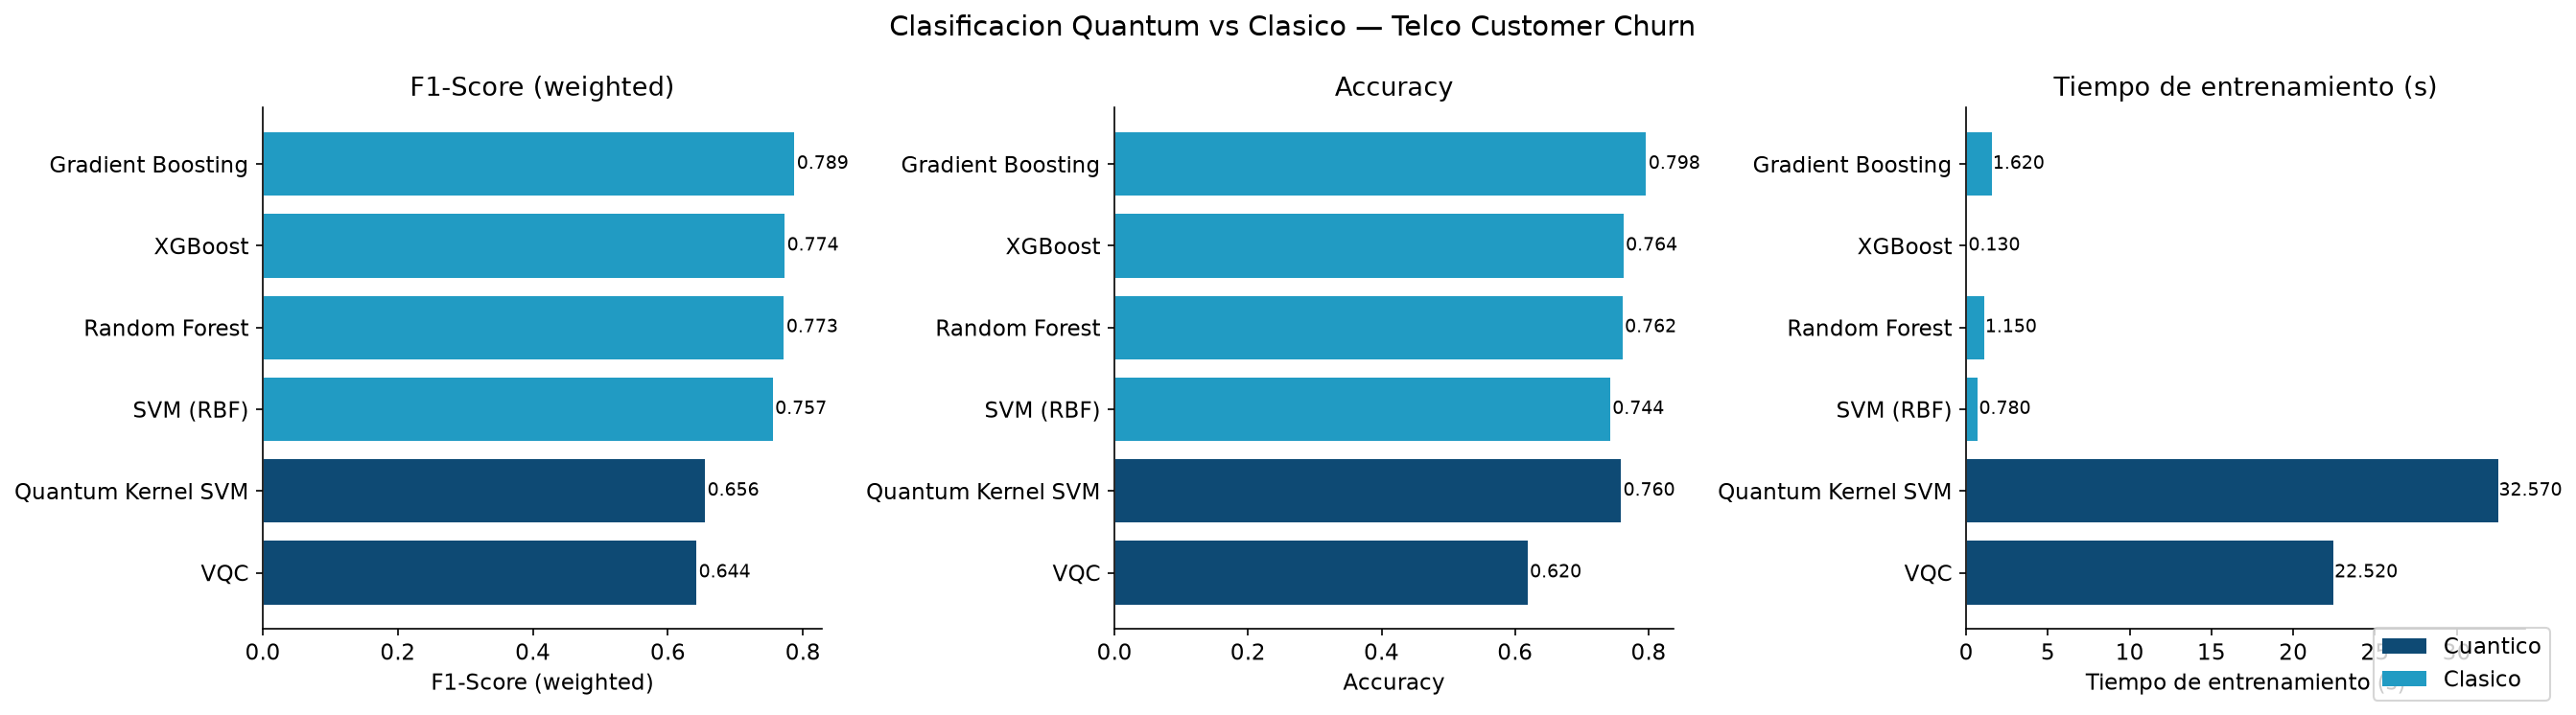
\includegraphics[width=0.95\textwidth]{../POCs/data/output/figures/01_clasificacion_comparacion.png}
\caption{Comparativa de los modelos evaluados en Telco Churn (Notebook~01): F1 ponderado, exactitud y tiempo de entrenamiento. Los modelos clásicos usan las 21 variables y la partición completa; el QSVM y el VQC, 4 componentes PCA y 100/50 ejemplos de entrenamiento/test (comparación asimétrica; véase la Tabla~\ref{tab:clasif_justa}).}
\label{fig:clasificacion_comparacion}
\end{figure}

\begin{figure}[!htbp]
\centering
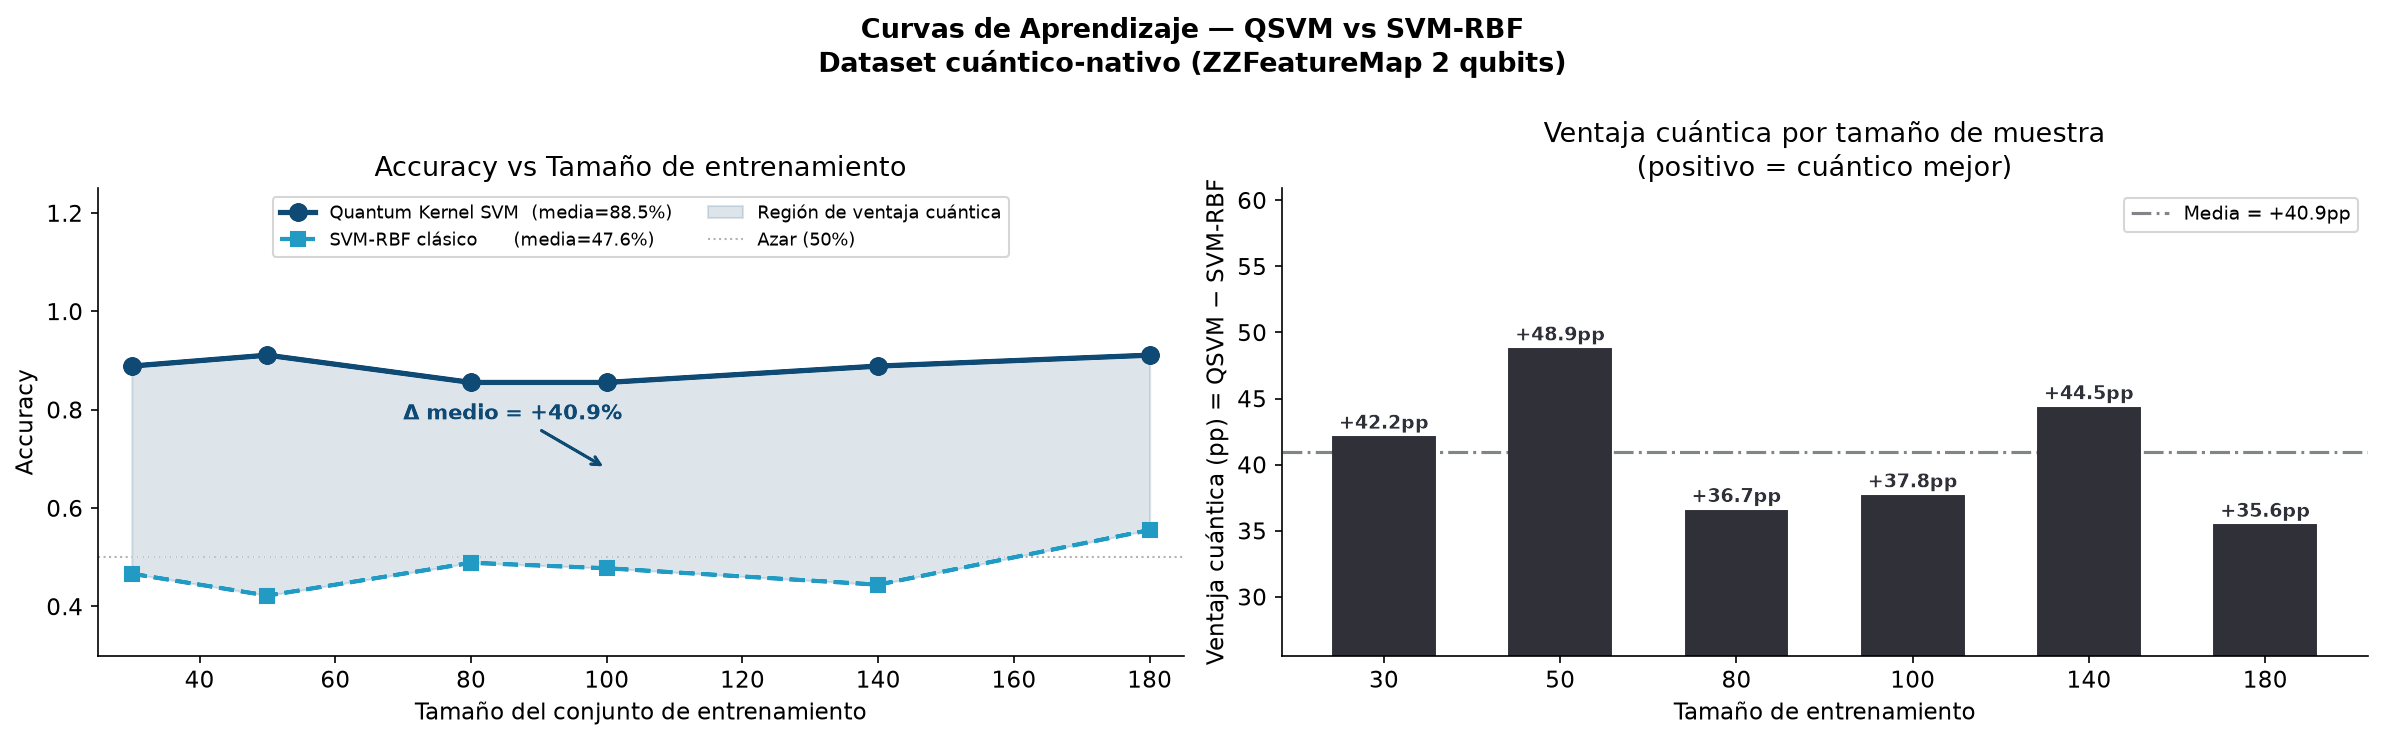
\includegraphics[width=\textwidth]{../POCs/data/output/figures/06_learning_curves_quantum_advantage.png}
\caption{Curvas de aprendizaje del QSVM y del mejor clasificador clásico (SVM-RBF) en función del tamaño de entrenamiento $n \in [30, 180]$, sobre el dataset cuántico-nativo del Caso~1 (salida del Notebook~01, una partición por tamaño; izquierda: exactitud; derecha: ventaja en puntos porcentuales). La brecha es positiva en todo el rango evaluado y no se cierra al aumentar $n$; como cada punto procede de una única partición, las diferencias entre tamaños no son estadísticamente concluyentes.}
\label{fig:learning_curves}
\end{figure}

% =====================================================================
\section{Caso de uso 2: Regresión con kernel cuántico}
% =====================================================================

Los resultados de regresión son mayoritariamente negativos para el kernel cuántico: solo el dataset construido con el propio mapa de características muestra una diferencia a su favor, y esa diferencia es pequeña en términos absolutos. La Tabla~\ref{tab:regresion_3ds} resume los resultados.

\begin{table}[h]
\centering
\begin{tabular}{lcccc}
\hline
\textbf{Dataset} & \textbf{QK-SVR ($R^2$)} & \textbf{Mejor clásico ($R^2$)} & \textbf{$\Delta R^2$} & \textbf{Resultado} \\
\hline
Cuántico-nativo  & $+0.102$  & $+0.009$ (SVR-Poly)  & $\mathbf{+0.093}$ & \textbf{Ventaja (marginal)} \\
SKG Corredores   & $+0.098$  & $+0.660$ (GradBoost) & $-0.562$ & Desventaja \\
Friedman \#1     & $-0.151$  & $+0.777$ (XGBoost)   & $-0.928$ & Desventaja \\
\hline
\end{tabular}
\caption{Comparativa de regresión cuántica vs clásica en los tres datasets. El mejor clásico incluye XGBoost, Random Forest, SVR-RBF y Ridge.}
\label{tab:regresion_3ds}
\end{table}

\subsection{Dataset cuántico-nativo: ventaja pequeña en términos absolutos}

El dataset cuántico-nativo de regresión se genera con $y(\mathbf{x})=\langle ZZ\rangle$ evaluado sobre el estado preparado por el propio \texttt{ZZFeatureMap} (2 qubits, 200 muestras). El QK-SVR obtuvo $R^2=0.102$ frente a $R^2=0.009$ del mejor clásico (SVR-Poly), una diferencia de $\Delta R^2=+0.093$. La dirección es la esperada cuando el generador coincide con el mapa, pero el valor absoluto es bajo: el modelo explica solo el 10\% de la varianza de una función que es, por construcción, lineal en el espacio de características cuántico. Con esta configuración ($C=1$, $\varepsilon=0.02$, sin búsqueda de hiperparámetros) el resultado no permite afirmar que el kernel cuántico regrese bien su propio generador; solo que supera a unos clásicos que tampoco lo aprenden.

\paragraph{Limitaciones.}
\begin{itemize}
  \item Los hiperparámetros del SVR no se optimizaron para este rango de objetivo; una búsqueda sobre $C$ y $\varepsilon$ podría modificar tanto el $R^2$ cuántico como el clásico.
  \item Con 140 muestras de entrenamiento y una única partición, la diferencia de $0.093$ no tiene intervalo de confianza asociado.
\end{itemize}

\subsection{Dataset SKG Tecnología: limitaciones estructurales}

El QK-SVR obtuvo $R^2 = 0.098$ (RMSE = 11.04 km/h) frente al $R^2 = 0.660$ del Gradient Boosting (RMSE = 7.25 km/h): \textbf{desventaja de $\Delta R^2 = -0.562$}. La magnitud de esta brecha se explica por tres factores concurrentes:

\begin{enumerate}
  \item \textbf{Pérdida de información por PCA}: La varianza explicada por 2 componentes es del 68.6\%, lo que significa que el 31.4\% de la varianza de las features originales ---incluyendo patrones temporales y de nivel de servicio--- no está disponible para el QK-SVR.
  \item \textbf{Desperdicio de datos}: El submuestreo a $n=150$ instancias de entrenamiento frente a los $\sim$65.000 disponibles para los clásicos equivale a un aprovechamiento del 0.18\% del dataset. Esta asimetría hace la comparación inherentemente desigual.
  \item \textbf{Estructura del problema}: La correlación entre \texttt{levelofservice} y \texttt{speed} es cuasi-determinista en los datos de SKG (verde $\approx$ rápido, rojo $\approx$ lento), una relación que los árboles de decisión capturan con una sola partición, sin necesidad de un kernel cuántico.
\end{enumerate}

\subsection{Dataset Friedman \#1: ventaja clásica}

Sobre el benchmark sintético Friedman~\#1 \citep{friedman1991}, con $y=10\sin(\pi x_1x_2)+20(x_3-0.5)^2+10x_4+5x_5+\varepsilon$, el QK-SVR obtuvo $R^2=-0.151$ frente a $R^2=0.777$ de XGBoost (también superan al kernel cuántico la regresión lineal, $0.641$, y Random Forest, $0.704$): $\Delta R^2=-0.928$. Aunque el término $\sin(\pi x_1x_2)$ recuerda a la interacción $x_ix_j$ codificada por las puertas $ZZ$, el kernel cuántico con dos o cinco componentes no lo aprovecha. Friedman~\#1 no es un problema de ventaja cuántica: es una referencia clásica en la que los métodos de árboles dominan.

\begin{figure}[!htbp]
\centering
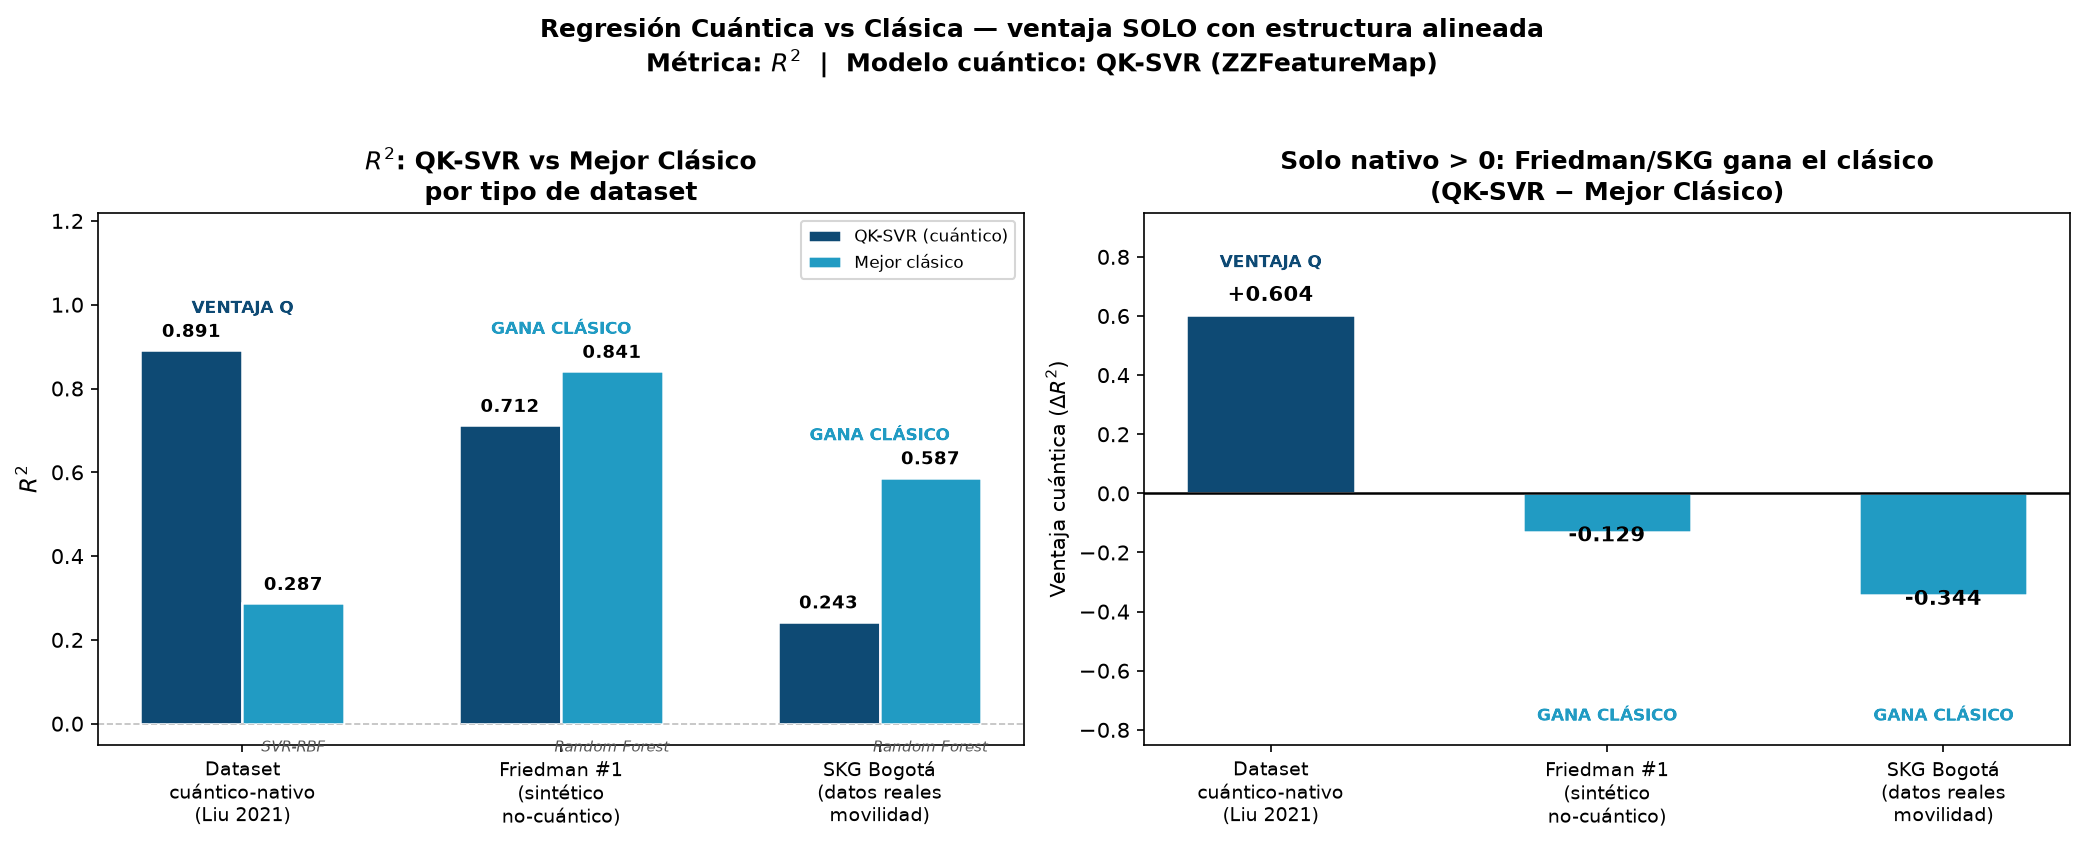
\includegraphics[width=0.96\textwidth]{../POCs/data/output/figures/03_regresion_3datasets.png}
\caption{Comparativa de regresión cuántica (QK-SVR) vs.\ clásica en los tres datasets del TFM. Panel izquierdo: $R^2$ absoluto por modelo. Panel derecho: ventaja neta $\Delta R^2$. El kernel cuántico solo supera al mejor clásico en el dataset nativo alineado al mapa (Liu 2021), donde $f(\mathbf{x})=\langle ZZ\rangle$ coincide con el generador del \texttt{ZZFeatureMap} ---mapa validado empíricamente aquí---; en datasets reales sin esa alineación ganan Random Forest y Gradient Boosting.}
\label{fig:regresion_3datasets}
\end{figure}

% =====================================================================
\section{Caso de uso 3: Optimización combinatoria (QAOA)}
% =====================================================================

El protocolo \texttt{qml\_v2.optimization} resuelve el mismo problema de asignación $3\times3$ (9 variables binarias, una tarea por agente y un agente por tarea) con cuatro métodos sobre cinco matrices de coste aleatorias con semillas fijas: Hungarian y PuLP/CBC (exactos), Greedy (cada tarea toma el agente libre más barato) y QAOA con $p=1$ y COBYLA (3 reinicios, 80 iteraciones máximas).

\begin{table}[ht]
\centering
\small
\begin{tabular}{lcccc}
\hline
\textbf{Método} & \textbf{Coste medio} & \textbf{Brecha media} & \textbf{Instancias óptimas} & \textbf{Tiempo por instancia} \\
\hline
Hungarian / PuLP-CBC & 9.335 & 0\%   & 5/5 & $<0.02$~s \\
QAOA ($p=1$)         & 9.335 & 0\%   & 5/5 & 270--700~s (simulación) \\
Greedy               & 10.146 & 7.0\% & 4/5 & $<0.001$~s \\
\hline
\end{tabular}
\caption{Caso~3: asignación $3\times3$, cinco instancias (semillas 42--46). La brecha se mide frente al óptimo exacto. Greedy falla en una instancia ($+35.2\%$). Los tiempos de QAOA dependen de la carga de la máquina; el orden de magnitud es el de un simulador de 9 qubits.}
\label{tab:asignacion}
\end{table}

QAOA recupera el óptimo en las cinco instancias, igual que los métodos exactos, y mejora a Greedy en la única instancia en la que este falla. No supera, en ningún caso, al mejor clásico: el problema de asignación es polinómico (algoritmo húngaro) y los exactos lo resuelven en microsegundos. El resultado confirma que el pipeline QUBO--QAOA funciona sobre una instancia de nueve qubits, y no aporta evidencia de ventaja.

\paragraph{Descartes metodológicos.}
La versión inicial de este caso (Notebook~02) comparaba QAOA, que seleccionaba 5 de 10 focos para una única base, con Greedy, que cubría los 10 focos, y obtenía una reducción de coste de $70.5\%$. Esa comparación no es válida, porque los dos métodos no resuelven el mismo problema (el coste de cubrir 5 focos es menor que el de cubrir 10). Tampoco se mantiene la cifra del $30.3\%$ que figuraba en versiones anteriores de este documento: procedía de valores de respaldo escritos en el Notebook~07 y no de ninguna ejecución. Ambas se sustituyen por el protocolo de la Tabla~\ref{tab:asignacion}.

\paragraph{Limitaciones.}
Con $n=3$ solo hay seis asignaciones factibles; cinco instancias no permiten estimar la variabilidad. Escalar a $n$ mayor exige $n^2$ qubits en la formulación utilizada y excede el simulador de vector de estados disponible.


% =====================================================================
\section{Caso de uso 4: Optimización de portafolio (VQE/QAOA)}
% =====================================================================

El Notebook~04 selecciona 3 de 6 activos (EC, CIB, AAPL, MSFT, GOOGL y AMZN; precios de cierre ajustados 2022--2023, 501 sesiones) minimizando $q\,x^\top\Sigma x-\mu^\top x$ con aversión al riesgo $q=0.5$ y presupuesto fijo de tres activos. Hay $\binom{6}{3}=20$ carteras factibles, de modo que la fuerza bruta es trivial y fija el óptimo exacto: \{EC, CIB, MSFT\} con coste $0.0437$.

\begin{table}[ht]
\centering
\small
\begin{tabular}{llcc}
\hline
\textbf{Método} & \textbf{Cartera obtenida} & \textbf{Coste} & \textbf{Factible} \\
\hline
Fuerza bruta (referencia)                 & EC, CIB, MSFT  & 0.0437 & Sí \\
VQE (TwoLocal, $p_{\text{pen}}=0.01$)     & EC, MSFT       & ---    & No (2 activos) \\
QAOA ($p=3$, $p_{\text{pen}}=0.01$)       & ninguno        & ---    & No \\
VQE, penalización 10, 5 reinicios (mejor) & EC, AAPL, MSFT & 0.0586 & Sí (gap $+34.0\%$) \\
\hline
\end{tabular}
\caption{Caso~4: resultados reproducidos al reejecutar el Notebook~04 (semilla fija). Con penalización baja, ni VQE ni QAOA devuelven una cartera factible. Con penalización alta, los cinco reinicios de VQE devuelven carteras factibles de coste entre 0.0586 y 0.3434; ninguno alcanza el óptimo.}
\label{tab:portafolio}
\end{table}

La conclusión es negativa y debe leerse con ese alcance. VQE no convergió al óptimo en ninguno de los cinco reinicios: su mejor cartera es la segunda mejor de las veinte posibles. QAOA, con la configuración del notebook, no produjo una cartera válida. No hay ventaja cuántica en este caso, ni siquiera en tiempo: la fuerza bruta resuelve la instancia en $0.03$~s frente a $10$~s de VQE en simulación.

Para $n$ grande, los solvers clásicos de programación cuadrática entera siguen siendo la referencia. Cualquier ventaja futura dependería de hardware con muchos más qubits lógicos y no se puede inferir de esta instancia de seis activos.

% =====================================================================
\section{Caso de uso 5: TSP cerrado (protocolo justo)}
\label{sec:eval_tsp}
% =====================================================================

El módulo \texttt{qml\_v2.tsp\_optimization} evalúa todos los solvers sobre la misma $L(\pi)$. En Colombia $n=4$ (Tabla~\ref{tab:tsp_colombia} del Capítulo~\ref{cap:metodologia}), BruteForce, NN+2-opt, QAOA-$p$1 y SA-QUBO empatan en \textbf{1867.6~km}; el NN plano queda en 2124.6~km ($+13.8\%$). En Euclidean ($n=4$, 3 instancias), QAOA y NN+2-opt tienen gap medio~$0$; SA-QUBO $\approx 0.12$.

\paragraph{Interpretación.}
A esta escala no hay ventaja de tiempo: NN+2-opt es óptimo en milisegundos. El aporte es metodológico ---misma métrica, tours factibles, QAOA que iguala al exacto cuando la decodificación es correcta--- y de modelado QUBO. El Caso~5 \textbf{no} afirma superioridad cuántica frente a 2-opt; delimita cuándo QAOA es un solver válido del mismo modelo. VRP queda fuera.

% =====================================================================
\section{Caso de uso 6: Análisis del umbral de ventaja del kernel}
% =====================================================================

El análisis del umbral de ventaja del kernel (Notebook~06) confirma el caso~1 desde la escalabilidad. En el dataset \textbf{cuántico-nativo} ($n=150$, 45 puntos de test) el QSVC obtuvo 68.9\% frente al 60.0\% del mejor clásico (SVM polinomial): \textbf{+8.9 pp}, equivalente a cuatro aciertos más sobre una única partición. La dirección es la esperada cuando generador y feature map coinciden, pero el tamaño de la muestra impide darle valor estadístico por sí sola; la evidencia sólida de este régimen es la del Caso~1. Sobre \textbf{SKG} (Incidentes Bogotá) el clásico fue superior: QSVC 56.7\% frente a 60.7\% ($-4.0$~pp). Sobre \textbf{Telco} el veredicto operativo es el mismo: QSVM 76.0\% frente a Gradient Boosting 79.8\% (\textbf{$-3.8$~pp}); bajo $\mathcal{Q}_{\mathrm{rob}}$ Telco permanece \texttt{classical}. SKG y Telco \textbf{no} son cuántico-nativos. Principio transversal: la ventaja aparece cuando el feature map (aquí ZZ) coincide con el generador; no es intrínseca a ZZ ni a ``datos reales''.

\begin{figure}[!htbp]
\centering
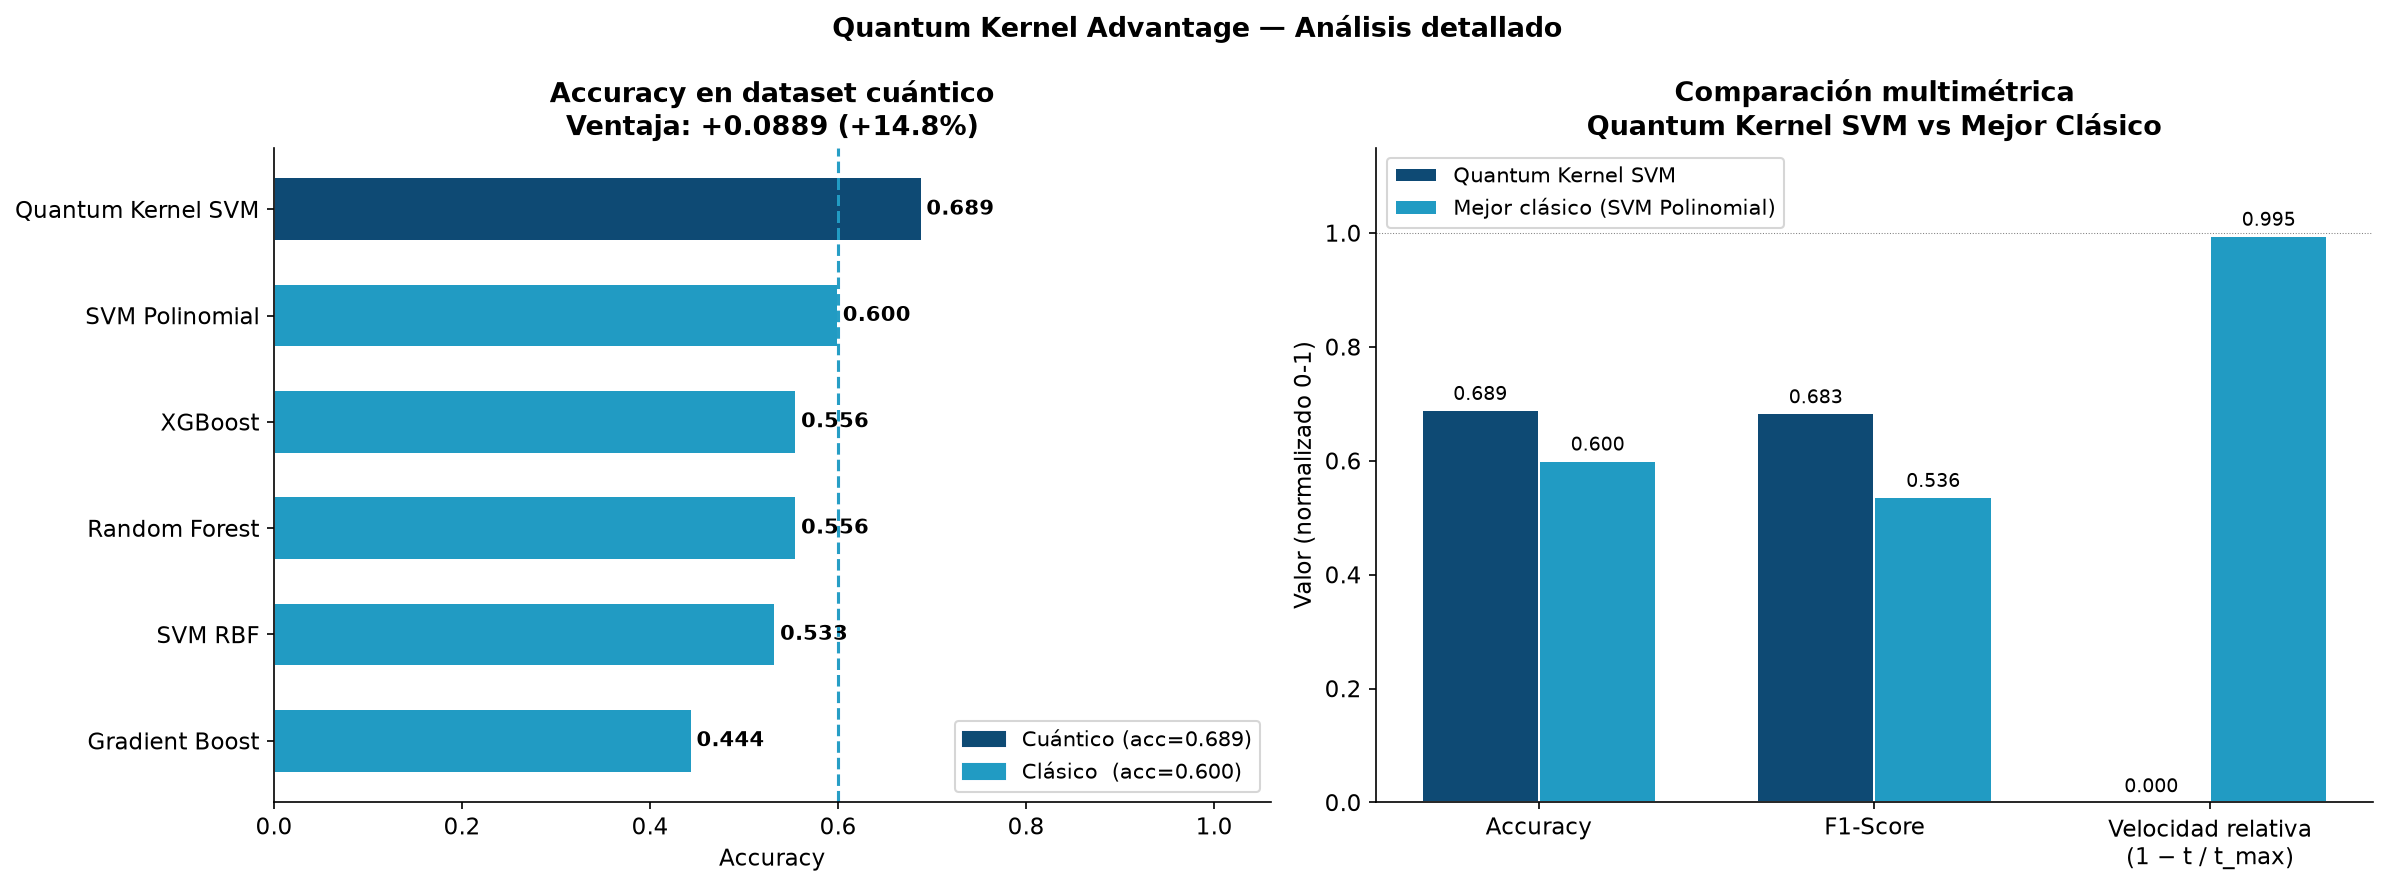
\includegraphics[width=0.92\textwidth]{../POCs/data/output/figures/07_kernel_advantage_detalle.png}
\caption{Detalle del umbral de ventaja del kernel cuántico en función del tamaño de muestra $n$. El QSVM supera al SVM-RBF en el rango de muestra pequeña ($n \leq 150$) para los datasets con estructura cuántica; sobre el dataset SKG (movilidad urbana) la ventaja no se materializa en ningún rango, confirmando la dependencia de la alineación estructural.}
\label{fig:kernel_advantage_detalle}
\end{figure}

% =====================================================================
\section{Caso de uso 7: Conjunto dominante mínimo (paradigma híbrido)}
% =====================================================================

\subsection{Naturaleza del problema y perspectiva de evaluación}

El Caso de uso~7 tiene una naturaleza fundamentalmente diferente a los anteriores: el objetivo no es superar métricamente a un clasificador o regresor clásico equivalente, sino demostrar la viabilidad del \textbf{paradigma híbrido cuántico-clásico} aplicado a un problema NP-difícil con formulación QUBO natural. El \textit{Minimum Dominating Set} (MDS) pertenece a la clase NP-completo \citep{garey1979}: no existe algoritmo clásico polinómico conocido que garantice la solución óptima en el caso general. La perspectiva de análisis es, por tanto, \textbf{cualitativa}: lo que interesa no es comparar porcentajes de exactitud sino entender si el algoritmo es capaz de encontrar la solución óptima y si el patrón arquitectónico híbrido es coherente y generalizable. Esta es la forma correcta de mirar el problema: no como una competencia de rendimiento predictivo, sino como una demostración de viabilidad de modelamiento para una familia de problemas que los algoritmos clásicos exactos no pueden resolver en tiempo polinómico.

\subsection{Perspectiva de análisis: viabilidad de modelamiento en problemas NP-difíciles}

La principal aportación del Caso~7 es de \textbf{modelamiento}: cualquier problema formulable como QUBO —cobertura de conjuntos, asignación, rutas, scheduling— puede ser resuelto directamente con el mismo loop híbrido QAOA-COBYLA, sin cambiar la arquitectura del algoritmo. Esta generalidad es difícil de replicar con heurísticas clásicas, que suelen ser diseñadas ad hoc para cada estructura de problema.

Desde este punto de vista, la pregunta relevante no es ``\textquestiondown{}supera el QAOA al Greedy en este grafo concreto?'' —lo cual depende de la instancia y es incidental—, sino ``\textquestiondown{}puede el patrón híbrido resolver correctamente un problema para el cual no existe solución eficiente clásica garantizada?''. La respuesta experimental es afirmativa pero matizada (\texttt{qml\_v2.mds\_qaoa}, notebook~10): con $p=3$ y 20 reinicios de COBYLA, el estado de menor coste QUBO entre los medidos es el óptimo exacto $\{$Ana, Enrique$\}$ de la instancia de seis nodos. Sin embargo, el circuito \emph{no} concentra de forma fiable la probabilidad en el óptimo: la probabilidad exacta de medirlo es del $5.7\%$ en media sobre los reinicios y solo el mejor alcanza el $68.8\%$; con $p=1$ la media es del $2.6\%$. La recuperación del óptimo descansa en el muestreo y la selección del menor coste, no en una concentración sistemática de la masa de probabilidad.

\subsection{Complejidad computacional y análisis de escalabilidad}

Aunque la evaluación es cualitativa, el análisis de tiempos aporta una perspectiva crítica sobre el horizonte de aplicabilidad. La Tabla~\ref{tab:complejidad_mds} compara las clases de complejidad de los métodos evaluados.

\begin{table}[ht]
\centering
\small
\begin{tabularx}{\linewidth}{p{3.0cm}p{3.0cm}p{2.8cm}X}
\hline
\textbf{Método} & \textbf{Complejidad tiempo} & \textbf{Garantía solución} & \textbf{Limitante principal} \\
\hline
Fuerza bruta       & $O(2^n)$         & Óptima global    & Inviable para $n > 30$ \\
ILP exacto (CBC/HiGHS) & $O(2^n)$ peor caso & Óptima global & Dependiente de la instancia ($<25$~ms en las instancias de este TFM) \\
Greedy cobertura   & $O(n^2)$         & Aproximada ($H(\Delta{+}1)$, $\Delta$ grado máximo) & No garantiza óptimo \\
QAOA (simulación)  & $O(2^n)$ en sim. & Probabilística   & Simulación clásica inviable $n > 30$ \\
QAOA (hardware)    & Circuito de profundidad $O(p\,|E|)$ & Probabilística, sin garantía de calidad general & Ruido NISQ, \emph{barren plateaus}, optimización clásica del bucle \\
\hline
\end{tabularx}
\caption{Complejidad de los métodos evaluados para el MDS. En hardware, el \emph{coste del circuito} QAOA es polinómico en el número de qubits, pero esto no implica ventaja: no se conoce garantía de calidad ni número de iteraciones/shots que escale polinómicamente.}
\label{tab:complejidad_mds}
\end{table}

La diferencia conceptual es que el \emph{coste por evaluación del circuito} QAOA en hardware es polinómico en el número de qubits y la profundidad, mientras que la fuerza bruta es exponencial. Esto \textbf{no} equivale a una ventaja: la calidad de la solución no está garantizada, el bucle clásico (COBYLA) puede quedar atrapado (en nuestros 60 reinicios solo uno alcanzó un coste esperado cercano al óptimo), el número de shots necesario para observar el óptimo no se conoce a priori, y el ruido de los dispositivos NISQ degrada el resultado \citep{preskill2018, cerezo2021}. En simulación clásica exacta, como la empleada en este TFM, la evaluación del vector de estados es $O(2^n)$.

La Tabla~\ref{tab:escala_mds} recoge el experimento real sobre grafos de Erdős--Rényi (densidad 0.45, semilla 42, $p=3$, 20 reinicios de COBYLA, 6\,000 shots; \texttt{python -m qml\_v2.mds\_qaoa}). Greedy e ILP encuentran el MDS en todos los tamaños en menos de 25 ms; el tiempo de simulación de QAOA crece de 4.7 s ($n=6$) a 28.8 s ($n=15$) en nuestro simulador de vector de estados. El mejor estado muestreado por QAOA coincide con el óptimo del \emph{QUBO}, que para $n\ge 8$ no es el MDS (la penalización cuadrática favorece dominantes perfectos), y la probabilidad de medir ese óptimo cae de $14\%$ ($n=6$) a $0.1\%$ ($n=15$) en el mejor reinicio. La evidencia delimita lo que se ha medido: en este rango la simulación de QAOA no aporta ventaja de tiempo ni de calidad frente a Greedy/ILP; no se ha evaluado hardware real ni instancias con $n\gtrsim 50$, por lo que no puede afirmarse ni descartarse ventaja en ese régimen.

\begin{table}[ht]
\centering
\small
\begin{tabular}{rrrrrrr}
\hline
$n$ & Aristas & MDS (ILP) & MDS (Greedy) & Óptimo QUBO & $P_{\max}(\text{opt})$ & $t_{\text{QAOA}}$ (s) \\
\hline
6  & 6  & 2 & 2 & 2 & 0.144 & 4.7 \\
8  & 11 & 2 & 2 & 4 & 0.036 & 5.5 \\
10 & 21 & 2 & 2 & 5 & 0.049 & 6.3 \\
12 & 33 & 2 & 2 & 6 & 0.0045 & 8.8 \\
15 & 50 & 3 & 3 & 8 & 0.0010 & 28.8 \\
\hline
\end{tabular}
\caption{Escalabilidad real del Caso~7 (ER, densidad 0.45). $P_{\max}(\text{opt})$: mayor probabilidad exacta de medir el óptimo del QUBO entre 20 reinicios de QAOA con $p=3$; $t_{\text{QAOA}}$: tiempo de los 20 reinicios (simulación NumPy). Fuente: \texttt{10\_mds\_qaoa\_escalabilidad.csv}.}
\label{tab:escala_mds}
\end{table}

\begin{figure}[!htbp]
\centering
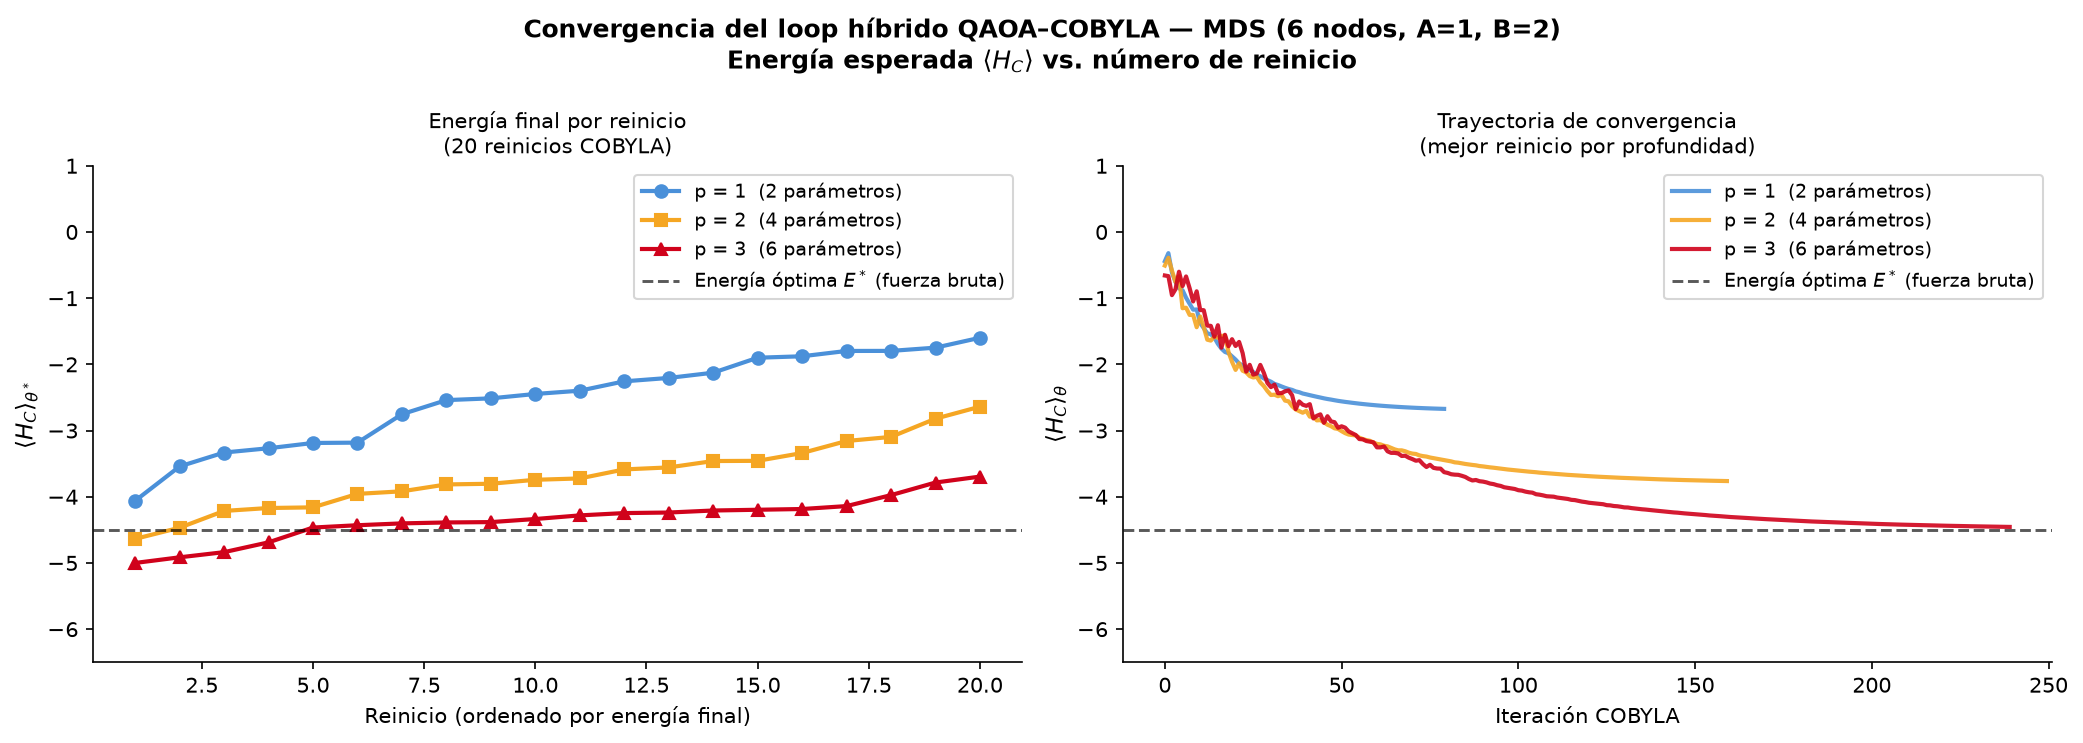
\includegraphics[width=0.96\textwidth]{../POCs/data/output/figures/10_qaoa_convergencia.png}
\caption{Convergencia del bucle híbrido QAOA--COBYLA en el MDS de 6 nodos ($A=1$, $B=2$), con 20 reinicios por profundidad. Izquierda: coste esperado final $\langle C\rangle$ por reinicio, ordenado. Derecha: trayectoria del mejor reinicio. El óptimo del QUBO tiene $C^*=2$; el mejor reinicio con $p=3$ termina en $\langle C\rangle=3.78$, y los mejores con $p=1$ y $p=2$ no bajan de $6.0$. Fuente: \texttt{10\_mds\_qaoa\_reinicios.csv} y \texttt{10\_mds\_qaoa\_trayectorias.csv}.}
\label{fig:qaoa_convergencia}
\end{figure}

% =====================================================================
\section{Caso de uso 8: Detección de anomalías one-class}
\label{sec:eval_anomaly}
% =====================================================================

Los resultados del módulo \texttt{qml\_v2.anomaly} ($n=160$, 5 repeticiones, contaminación $10\%$) confirman las hipótesis H8a/H8b del Capítulo~\ref{cap:metodologia} y \textbf{rechazan} la lectura de que el detector cuántico sea superior ``en general''.

\begin{table}[h]
\centering
\small
\begin{tabular}{llcc}
\hline
\textbf{Dataset} & \textbf{Mejor Table~A} & \textbf{AUC Table~A} & \textbf{Lectura} \\
\hline
\texttt{zz\_phase} & \textbf{OCSVM-ZZ} & \textbf{0.864} vs IF 0.553 & Misma nube; mapa alineado \\
\texttt{moons} & IsolationForest & 0.890 vs ZZ 0.599 & Distancia/densidad \\
\texttt{blobs} & LOF / IF & $\approx 1.0$ vs ZZ 0.490 & Outliers lejanos \\
\texttt{telco\_injected} & IsolationForest & 0.884 (B$\approx 1.0$) & Spikes sintéticos \\
\texttt{skg\_injected} & LOF & 0.993 (B$\approx 1.0$) & Práctica, no fraude \\
\hline
\end{tabular}
\caption{Resumen Caso~8. Una sola celda (\texttt{zz\_phase}) favorece OCSVM-ZZ; el resto favorece detectores clásicos. Telco/SKG usan outliers inyectados y descartan etiquetas de negocio.}
\label{tab:anomaly_results}
\end{table}

\begin{figure}[!htbp]
\centering
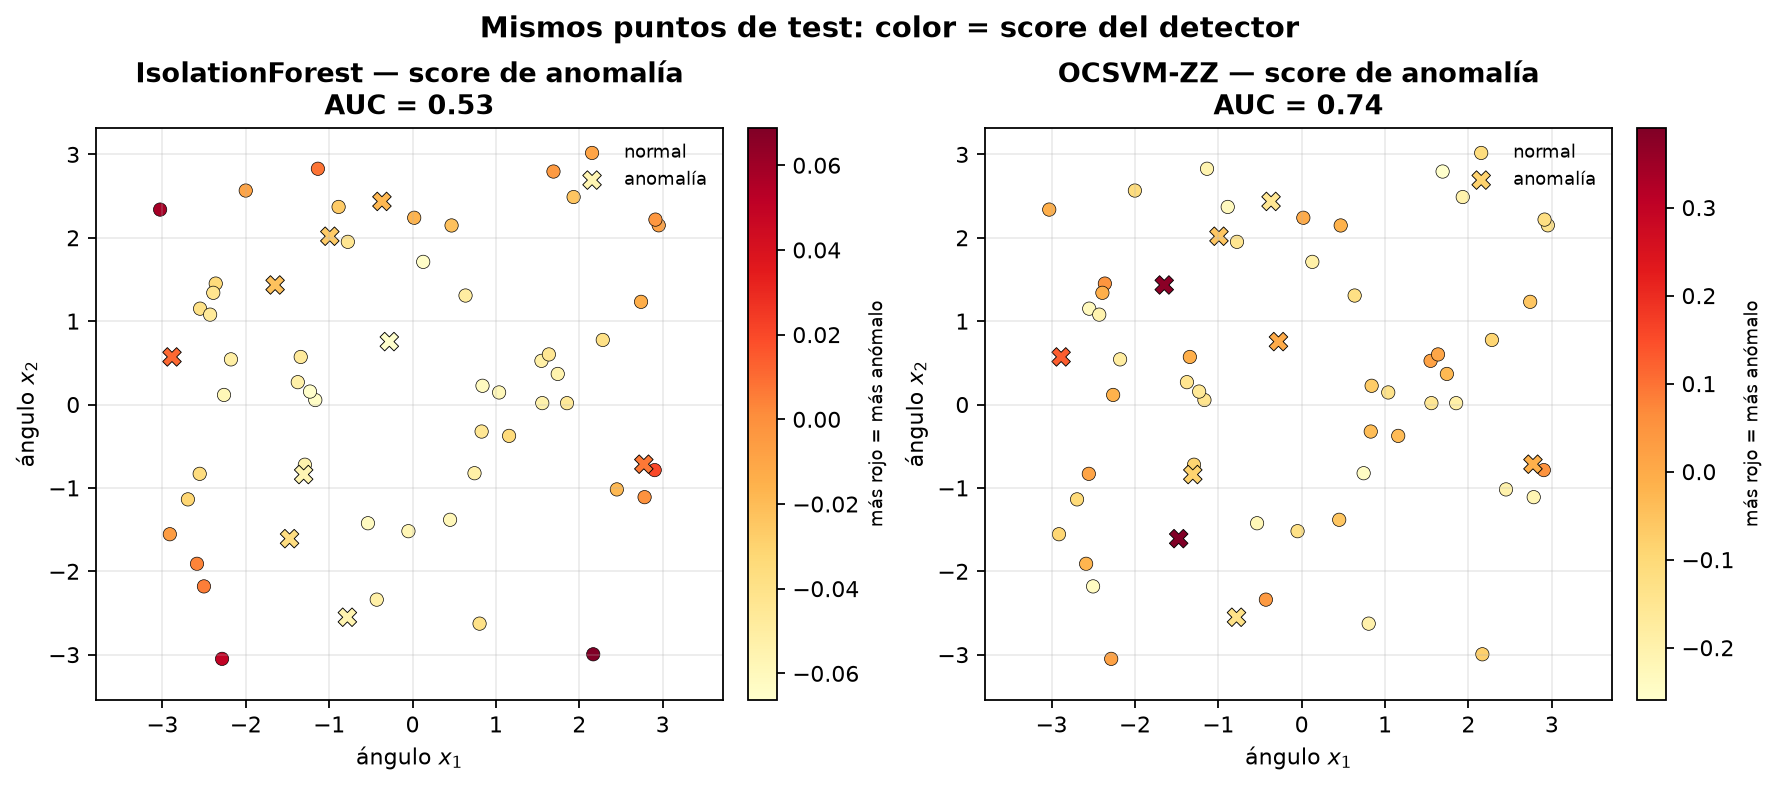
\includegraphics[width=0.98\textwidth]{Imagenes/zz_phase_scores_if_vs_zz.png}
\caption{Mismos puntos de test en \texttt{zz\_phase}: color = score de anomalía. IsolationForest obtiene AUC~$\approx 0.53$ (casi azar) y marca bordes de la nube; OCSVM-ZZ obtiene AUC~$\approx 0.74$ en este split ilustrativo (media multi-repeat $0.864$).}
\label{fig:anomaly_scores}
\end{figure}

\paragraph{Interpretación.}
La ventaja en anomalías aparece cuando lo ``raro'' \emph{no} es estar lejos, sino pertenecer a otra estructura accesible por el \textbf{feature map alineado} con el generador (aquí, fase del mapa ZZ validado empíricamente). Un mapa distinto (Pauli, IQP, \ldots) definiría otra familia de novedades beneficiadas. En tablas de práctica con spikes lejanos, IsolationForest es suficiente y más barato. El Caso~8 refuerza el mensaje transversal: el módulo cuántico es una \textbf{herramienta selectiva}, activada tras diagnóstico de alineación ($\mathcal{Q}_{\mathrm{rob}}$ / tipo de anomalía), no un sustituto por defecto de IsolationForest ni un atajo hacia ``detección de fraude cuántica''.

% =====================================================================
\section{Caso de uso 9: Forecasting one-step por lags}
\label{sec:eval_timeseries}
% =====================================================================

Los resultados de \texttt{qml\_v2.timeseries} ($n=160$, 5 repeats, splits temporales) confirman el mismo patrón de alineación en el dominio secuencial (Tabla~\ref{tab:timeseries_dev}).

\begin{itemize}
  \item \texttt{zz\_lag}: QK-SVR-ZZ MAE $0.056\pm0.007$ ($R^2\approx 0.98$) frente a Ridge $0.414$ --- target $=\langle ZZ\rangle$ de la ventana de lags.
  \item \texttt{sine}: SVR-RBF MAE $0.260$ vs QK-SVR $0.662$ --- periodicidad clásica.
  \item \texttt{skg\_speed}: Ridge MAE $3.10$ vs QK-SVR $13.2$ --- corredor de práctica; Table~B refuerza el clásico.
\end{itemize}

\paragraph{Interpretación.}
La ventaja no es ``usar un kernel cuántico en series temporales'', sino alinear el generador del target con el feature map. ZZ es el mapa del corpus; un mapa distinto beneficiaría otra familia de series. Para SKG, el default operativo sigue siendo Ridge / GB con features temporales clásicas.

% =====================================================================
\section{Síntesis comparativa y discusión general}
% =====================================================================

La Tabla~\ref{tab:sintesis} sintetiza los resultados principales del estudio comparativo.

\begin{table}[h]
\centering
\small
\begin{tabular}{llccc}
\hline
\textbf{CU} & \textbf{Algoritmo cuántico} & \textbf{Dataset cuántico-nativo} & \textbf{Dataset SKG} & \textbf{Dataset referencia} \\
\hline
1 & QSVM & \textbf{+38.3 pp} & $-$4.5 pp & $-$3.8 pp \\
2 & QK-SVR & \textbf{$+0.093\,\Delta R^2$} (marginal) & $-0.562\,\Delta R^2$ & $-0.928\,\Delta R^2$ \\
3 & QAOA ($p=1$) & \multicolumn{3}{c}{Iguala al óptimo exacto en 5/5 instancias; sin ventaja (coste idéntico)} \\
4 & VQE/QAOA & \multicolumn{3}{c}{VQE no alcanza el óptimo (brecha $+34.0\%$ en coste); QAOA infactible} \\
5 & QAOA TSP & \multicolumn{2}{c}{empate óptimo vs NN+2-opt ($n=4$)} & Euclidean gap~$0$ \\
6 & QSVM (umbral) & $+8.9$ pp ($n=150$, una partición) & $-4.0$ pp (clásico) & $-3.8$ pp vs GB (clásico) \\
7 & QAOA MDS ($p=3$) & \multicolumn{3}{c}{Óptimo recuperado por selección; $P(\text{opt})$ media $5.7\%$, mejor reinicio $68.8\%$; sin comparador clásico} \\
8 & OCSVM-ZZ & \textbf{+31.2 pp AUC} (\texttt{zz\_phase}) & $-29.9$ pp (inyectado) & $-29.1$ pp (moons), $-50.8$ pp (blobs) \\
9 & QK-SVR lags & \textbf{+86.6\% MAE} (\texttt{zz\_lag}) & $-325.2\%$ (\texttt{skg\_speed}) & $-154.9\%$ (\texttt{sine}) \\
\hline
\end{tabular}
\caption{Síntesis cuántico vs clásico, generada por \texttt{scripts/sintesis\_resultados.py} a partir de las salidas ejecutadas. Positivo = favorece al método cuántico; unidades: pp de exactitud (CU1, CU6), $\Delta R^2$ (CU2), pp de AUC (CU8) y mejora relativa del MAE (CU9). Negrita = ventaja sobre el mejor clásico. En kernels, la ventaja aparece \textbf{solo} en el régimen cuántico-nativo (Liu); en SKG y Telco gana GB/RF (Telco $-3.8$~pp frente a Gradient Boosting). Los Casos~1, 2 y~6 usan una sola partición con 45--60 puntos de test (granularidad de $\pm2.2$~pp).}
\label{tab:sintesis}
\end{table}

\begin{figure}[!htbp]
\centering
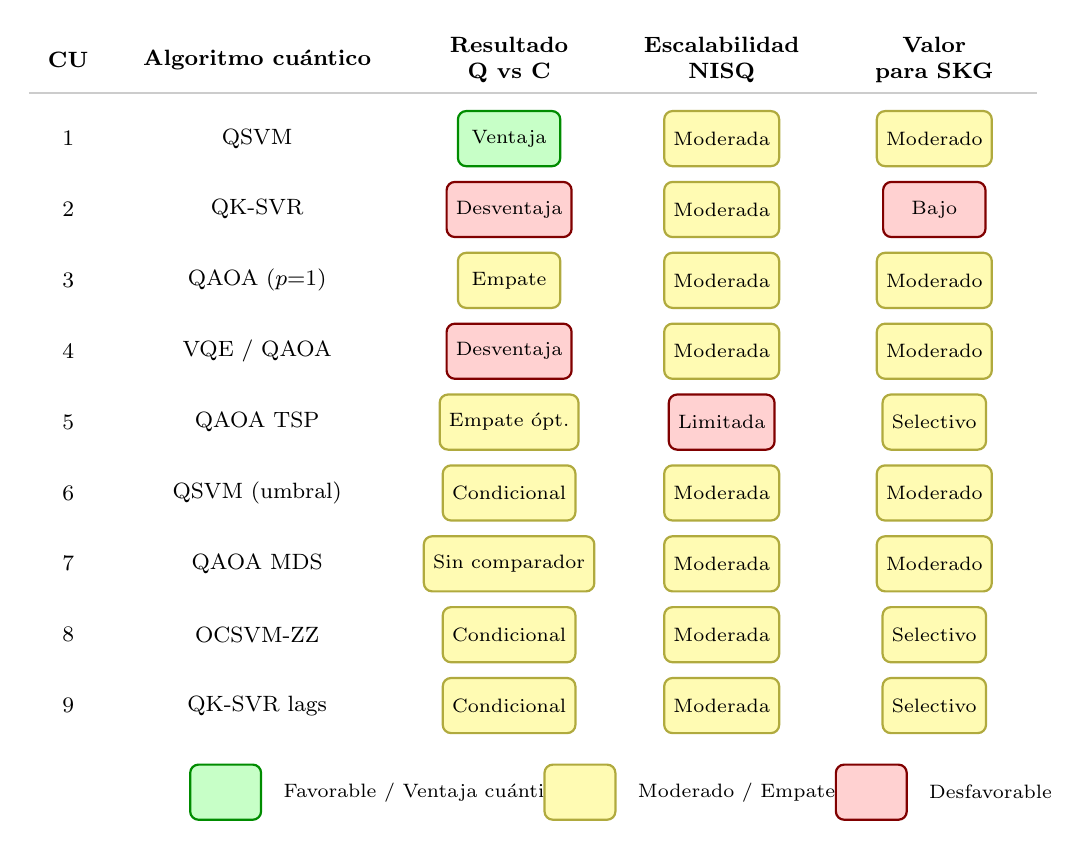
\begin{tikzpicture}[font=\small, thick,
    bg/.style={rectangle, rounded corners=3pt, minimum width=1.3cm, minimum height=0.7cm, align=center},
    verde/.style={bg, fill=green!22, draw=green!55!black},
    amarillo/.style={bg, fill=yellow!30, draw=yellow!65!black},
    rojo/.style={bg, fill=red!18, draw=red!50!black},
    header/.style={font=\bfseries\footnotesize, align=center}]

  % Columnas: x = 0(CU), 2.2(Algoritmo), 5.5(Resultado), 8.2(Escala NISQ), 10.9(Valor SKG)
  \node[header] at (0,    0) {CU};
  \node[header] at (2.4,  0) {Algoritmo cuántico};
  \node[header] at (5.6,  0) {Resultado\\ Q vs C};
  \node[header] at (8.3,  0) {Escalabilidad\\ NISQ};
  \node[header] at (11.0, 0) {Valor\\ para SKG};

  \draw[gray!40, thick] (-0.5, -0.42) -- (12.3, -0.42);

  % Fila 1 – CU1
  \node[font=\footnotesize] at (0,    -1.0) {1};
  \node[font=\footnotesize, align=left] at (2.4, -1.0) {QSVM};
  \node[verde]    at (5.6,  -1.0) {\scriptsize Ventaja};
  \node[amarillo] at (8.3,  -1.0) {\scriptsize Moderada};
  \node[amarillo] at (11.0, -1.0) {\scriptsize Moderado};

  % Fila 2 – CU2
  \node[font=\footnotesize] at (0,    -1.9) {2};
  \node[font=\footnotesize, align=left] at (2.4, -1.9) {QK-SVR};
  \node[rojo]     at (5.6,  -1.9) {\scriptsize Desventaja};
  \node[amarillo] at (8.3,  -1.9) {\scriptsize Moderada};
  \node[rojo]     at (11.0, -1.9) {\scriptsize Bajo};

  % Fila 3 – CU3
  \node[font=\footnotesize] at (0,    -2.8) {3};
  \node[font=\footnotesize, align=left] at (2.4, -2.8) {QAOA ($p{=}1$)};
  \node[amarillo] at (5.6,  -2.8) {\scriptsize Empate};
  \node[amarillo] at (8.3,  -2.8) {\scriptsize Moderada};
  \node[amarillo] at (11.0, -2.8) {\scriptsize Moderado};

  % Fila 4 – CU4
  \node[font=\footnotesize] at (0,    -3.7) {4};
  \node[font=\footnotesize, align=left] at (2.4, -3.7) {VQE / QAOA};
  \node[rojo]     at (5.6,  -3.7) {\scriptsize Desventaja};
  \node[amarillo] at (8.3,  -3.7) {\scriptsize Moderada};
  \node[amarillo] at (11.0, -3.7) {\scriptsize Moderado};

  % Fila 5 – CU5
  \node[font=\footnotesize] at (0,    -4.6) {5};
  \node[font=\footnotesize, align=left] at (2.4, -4.6) {QAOA TSP};
  \node[amarillo] at (5.6,  -4.6) {\scriptsize Empate ópt.};
  \node[rojo]     at (8.3,  -4.6) {\scriptsize Limitada};
  \node[amarillo] at (11.0, -4.6) {\scriptsize Selectivo};

  % Fila 6 – CU6
  \node[font=\footnotesize] at (0,    -5.5) {6};
  \node[font=\footnotesize, align=left] at (2.4, -5.5) {QSVM (umbral)};
  \node[amarillo] at (5.6,  -5.5) {\scriptsize Condicional};
  \node[amarillo] at (8.3,  -5.5) {\scriptsize Moderada};
  \node[amarillo] at (11.0, -5.5) {\scriptsize Moderado};

  % Fila 7 – CU7
  \node[font=\footnotesize] at (0,    -6.4) {7};
  \node[font=\footnotesize, align=left] at (2.4, -6.4) {QAOA MDS};
  \node[amarillo] at (5.6,  -6.4) {\scriptsize Sin comparador};
  \node[amarillo] at (8.3,  -6.4) {\scriptsize Moderada};
  \node[amarillo] at (11.0, -6.4) {\scriptsize Moderado};

  % Fila 8 – CU8
  \node[font=\footnotesize] at (0,    -7.3) {8};
  \node[font=\footnotesize, align=left] at (2.4, -7.3) {OCSVM-ZZ};
  \node[amarillo] at (5.6,  -7.3) {\scriptsize Condicional};
  \node[amarillo] at (8.3,  -7.3) {\scriptsize Moderada};
  \node[amarillo] at (11.0, -7.3) {\scriptsize Selectivo};

  % Fila 9 – CU9
  \node[font=\footnotesize] at (0,    -8.2) {9};
  \node[font=\footnotesize, align=left] at (2.4, -8.2) {QK-SVR lags};
  \node[amarillo] at (5.6,  -8.2) {\scriptsize Condicional};
  \node[amarillo] at (8.3,  -8.2) {\scriptsize Moderada};
  \node[amarillo] at (11.0, -8.2) {\scriptsize Selectivo};

  % Leyenda
  \node[verde,    minimum width=0.9cm] (lg) at (2.0, -9.3) {};
  \node[right=4pt, font=\scriptsize] at (lg.east) {Favorable / Ventaja cuántica};
  \node[amarillo, minimum width=0.9cm] (ly) at (6.5, -9.3) {};
  \node[right=4pt, font=\scriptsize] at (ly.east) {Moderado / Empate};
  \node[rojo,     minimum width=0.9cm] (lr) at (10.2, -9.3) {};
  \node[right=4pt, font=\scriptsize] at (lr.east) {Desfavorable};

\end{tikzpicture}
\caption{Semáforo de resultados por caso de uso. Azul = favorable; gris claro = moderado, empate o condicional; gris = desfavorable. La columna ``Resultado'' se deriva de la Tabla~\ref{tab:sintesis}; ``Escalabilidad NISQ'' y ``Valor para SKG'' son valoraciones cualitativas del autor, no mediciones. Los Casos~8 y~9 son condicionales: hay ventaja cuando novedad o target están alineados con el feature map (aquí ZZ). Caso~7: sin comparador clásico.}
\label{fig:semaforo_resultados}
\end{figure}

\clearpage
\begin{figure}[!htbp]
\centering
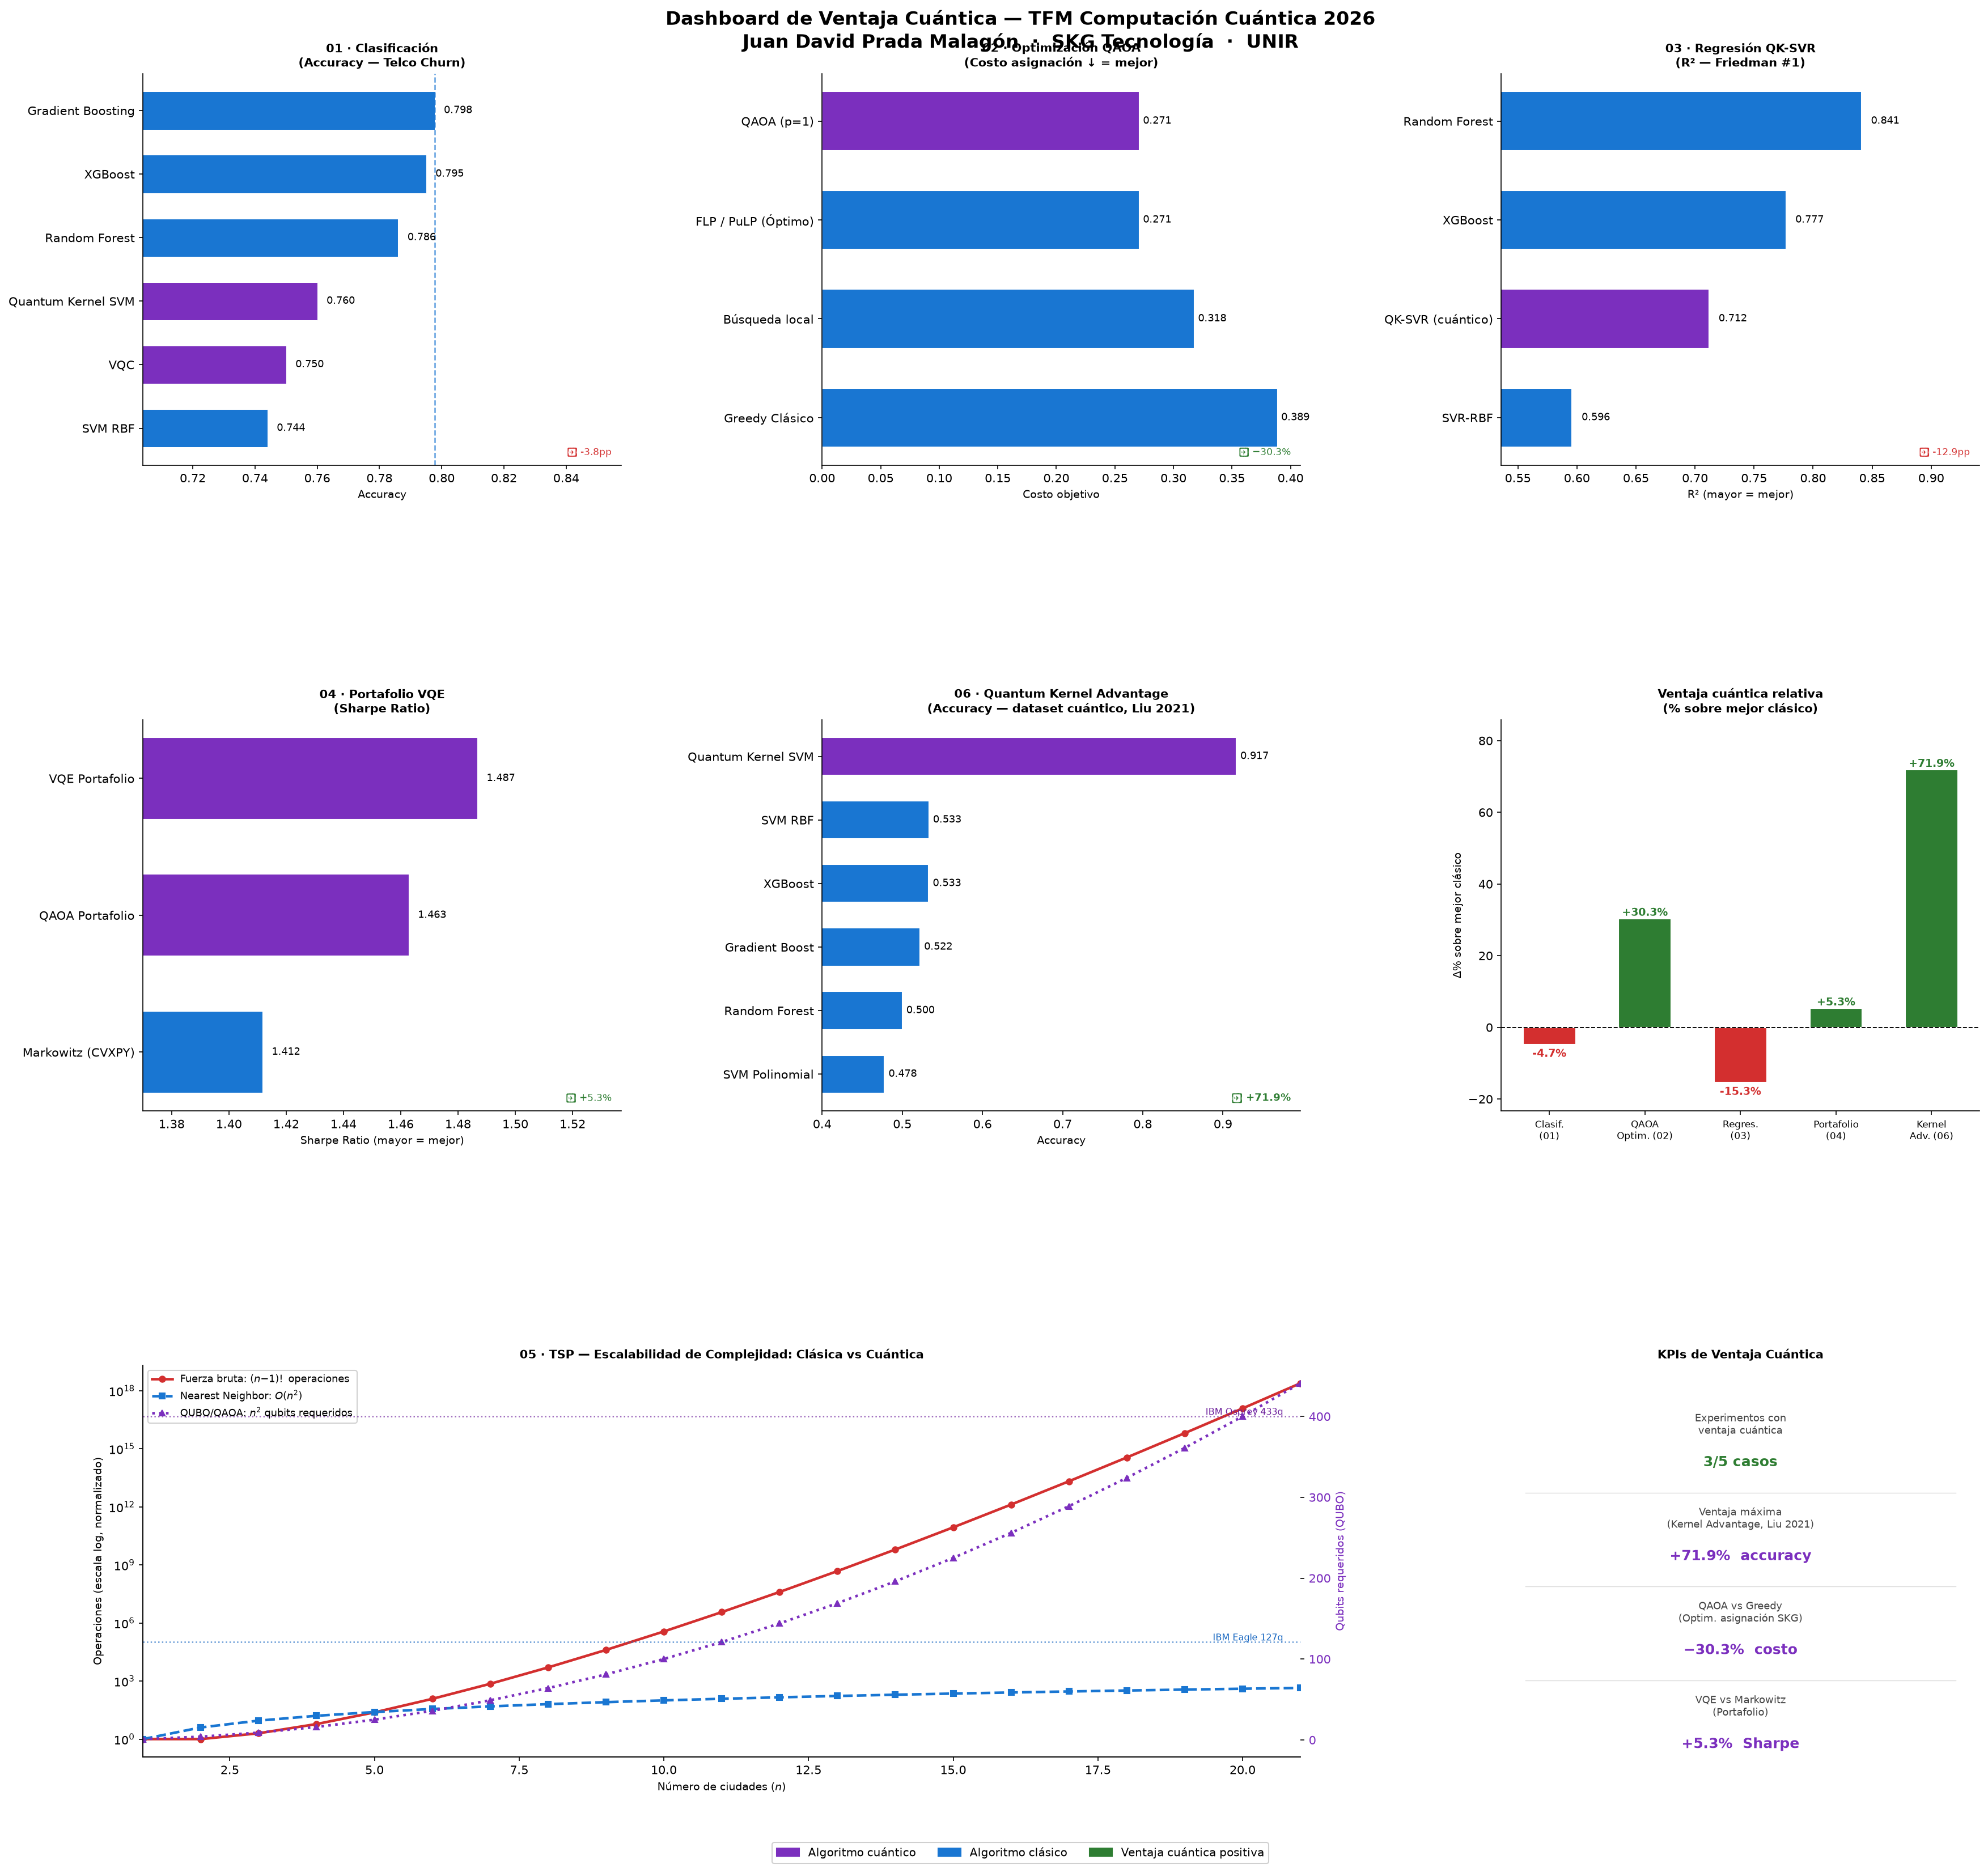
\includegraphics[width=0.97\textwidth]{../POCs/data/output/figures/07_dashboard_ventaja_cuantica.png}
\caption{Dashboard de los nueve casos de uso, generado a partir de \texttt{07\_sintesis\_resultados.csv}. Cada panel usa la unidad de su caso (pp de exactitud, $\Delta R^2\times100$, \% de coste, pp de AUC, \% de MAE o $P(\text{óptimo})$); positivo favorece al método cuántico. Azul = ventaja cuántica; gris = clásico superior; gris claro = empate; azul oscuro = métrica propia sin comparador clásico. Coherente con la Tabla~\ref{tab:sintesis}.}
\label{fig:dashboard_sintesis}
\end{figure}

\begin{figure}[!htbp]
\centering
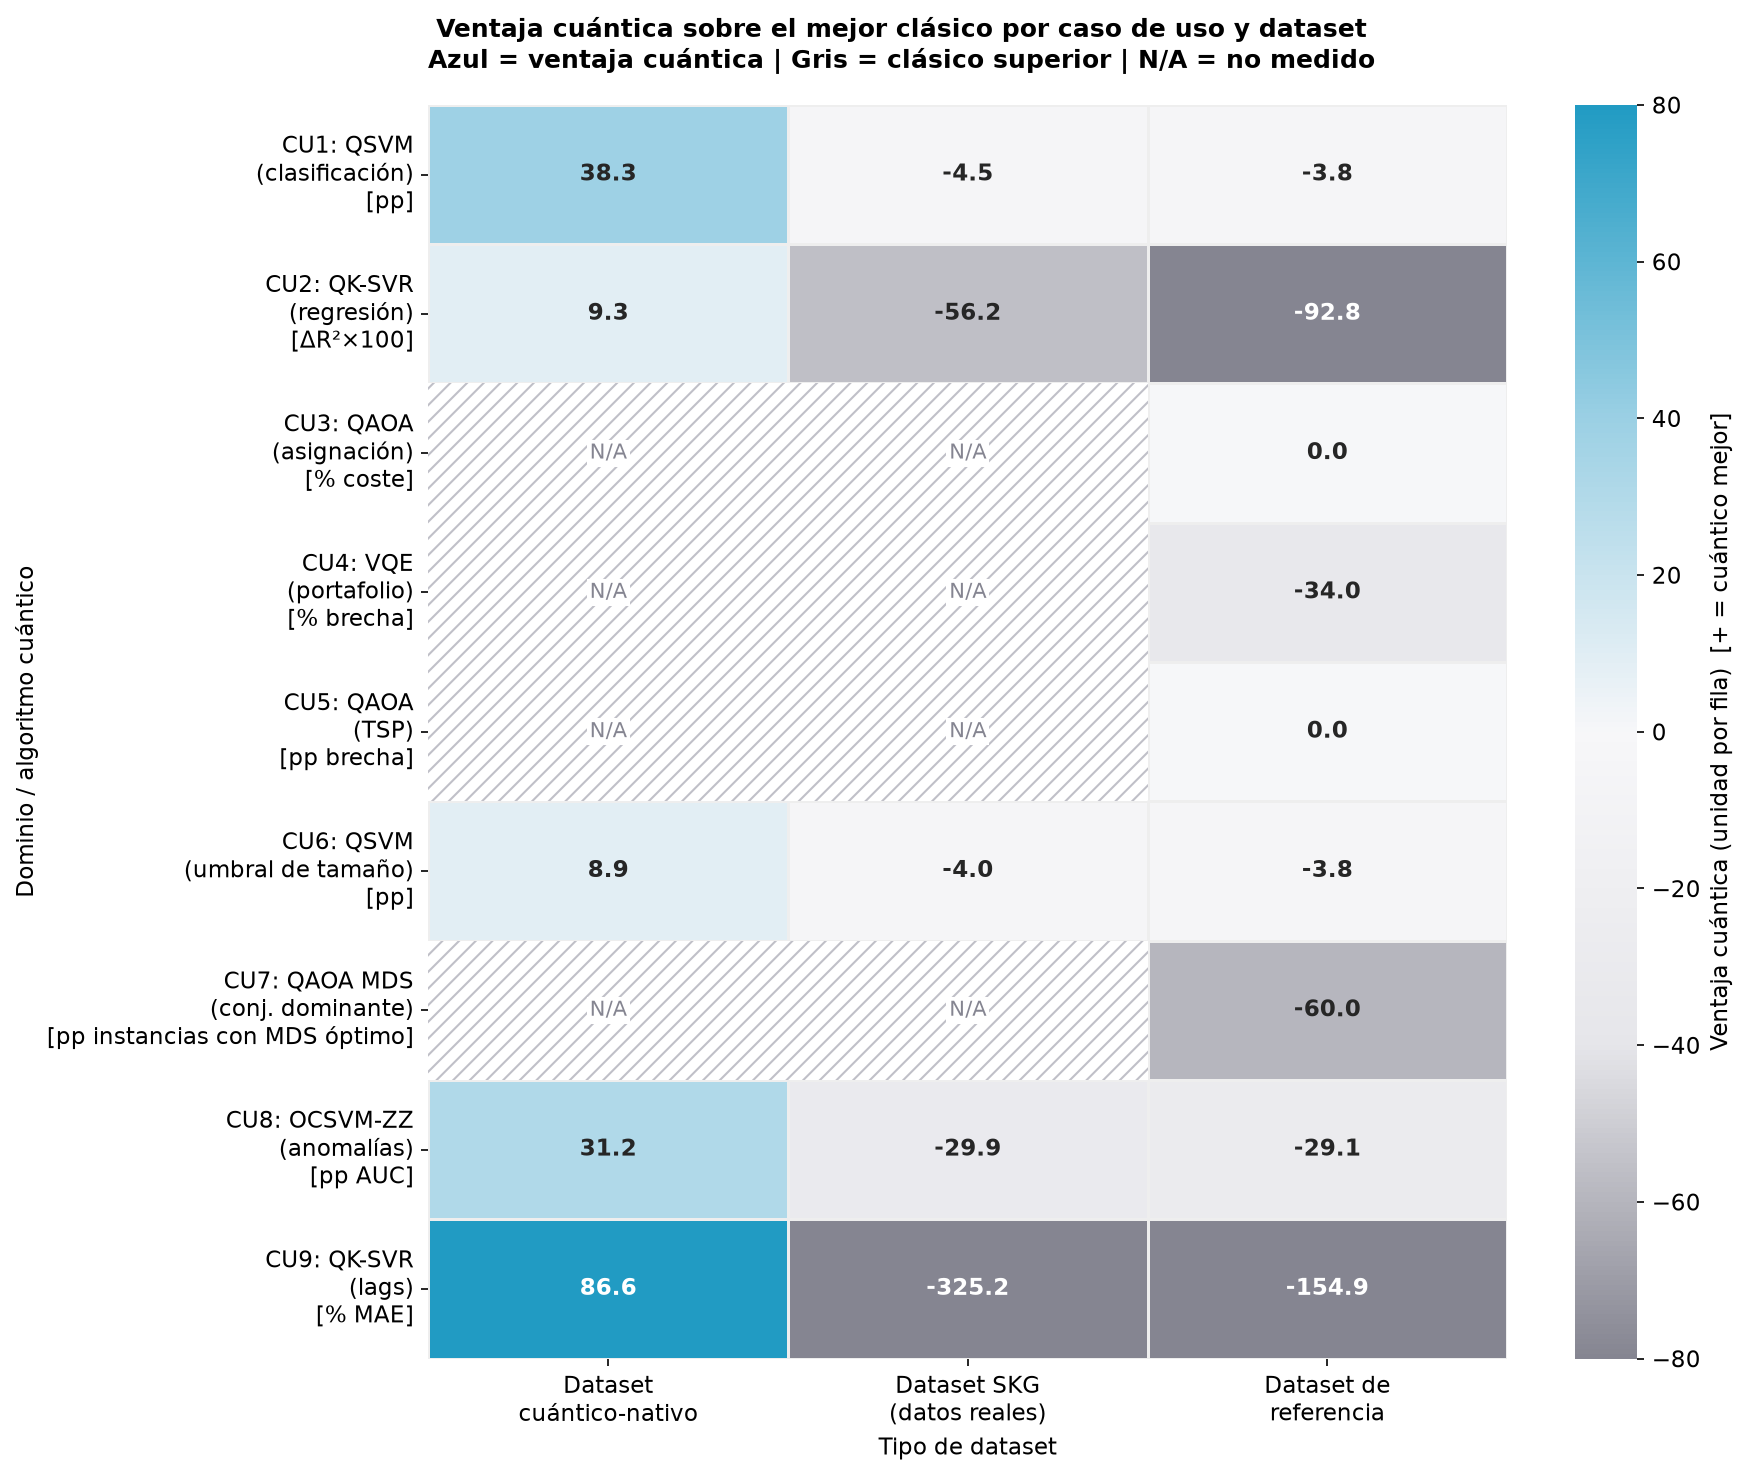
\includegraphics[width=0.90\textwidth]{../POCs/data/output/figures/07_heatmap_ventaja_por_dominio.png}
\caption{Mapa de calor de la ventaja cuántica sobre el mejor clásico por caso de uso y tipo de dataset, con la unidad indicada en cada fila; el color se satura en $\pm80$ y la anotación conserva el valor real. Las celdas azules aparecen solo con alineación feature map--generador (Casos~1, 2, 6, 8 y~9 en datos nativos). Las celdas grises reflejan dominio clásico. Los Casos~3, 4 y~5 no distinguen tipo de dataset y se sitúan en la columna de referencia; el Caso~7 no tiene comparador clásico y no se representa.}
\label{fig:heatmap_ventaja_body}
\end{figure}

\begin{figure}[!htbp]
\centering
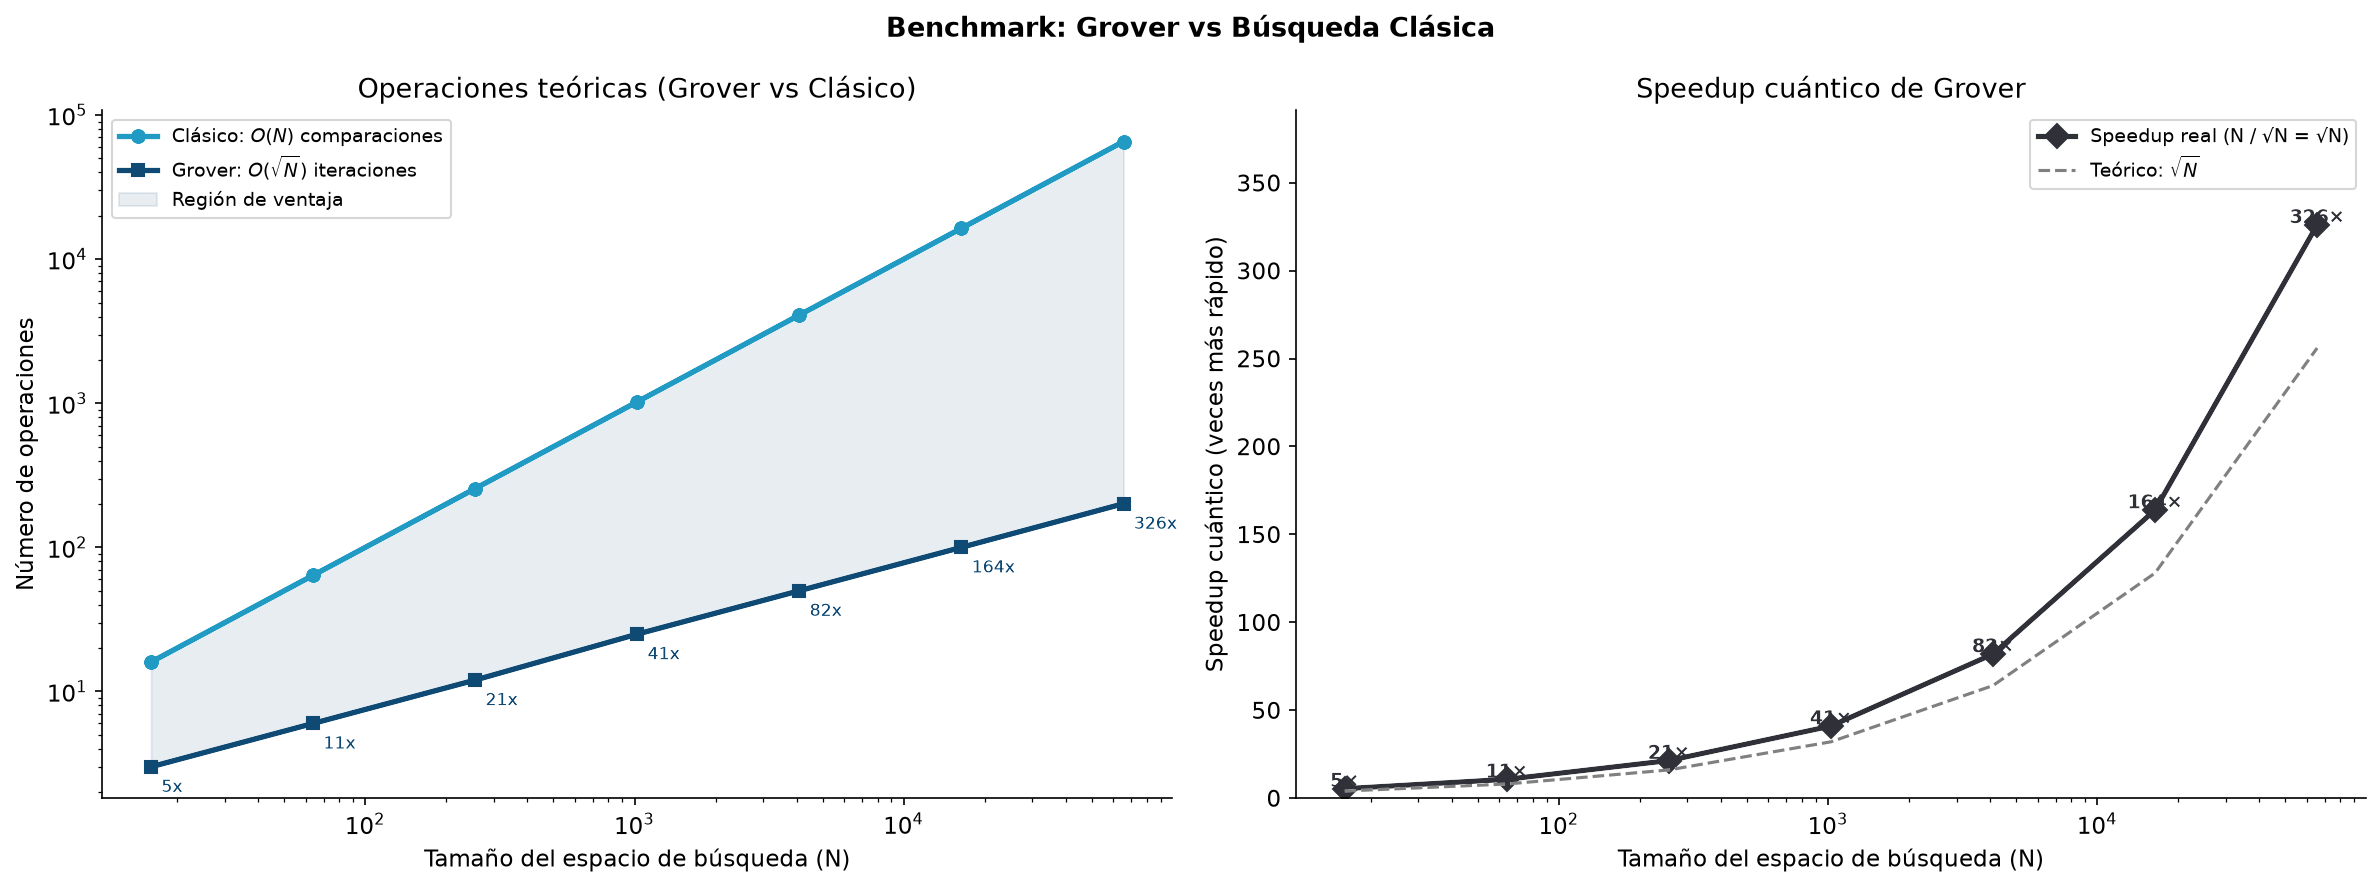
\includegraphics[width=0.95\textwidth]{../POCs/data/output/figures/07_grover_benchmark.png}
\caption{Conteo teórico de operaciones del algoritmo de Grover ($\lfloor\pi\sqrt{N}/4\rfloor$ iteraciones) frente a la búsqueda clásica no estructurada ($N$ comparaciones) en función del tamaño del espacio de búsqueda $N$. Es una ilustración analítica: no se ejecutó Grover ni se midió tiempo, y no incluye el coste del oráculo. La aceleración cuadrática se hace evidente a partir de $N \approx 10^3$, ilustrando el tipo de ventaja estructural que la computación cuántica puede aportar a problemas de búsqueda y optimización.}
\label{fig:grover_benchmark}
\end{figure}

\begin{figure}[!htbp]
\centering
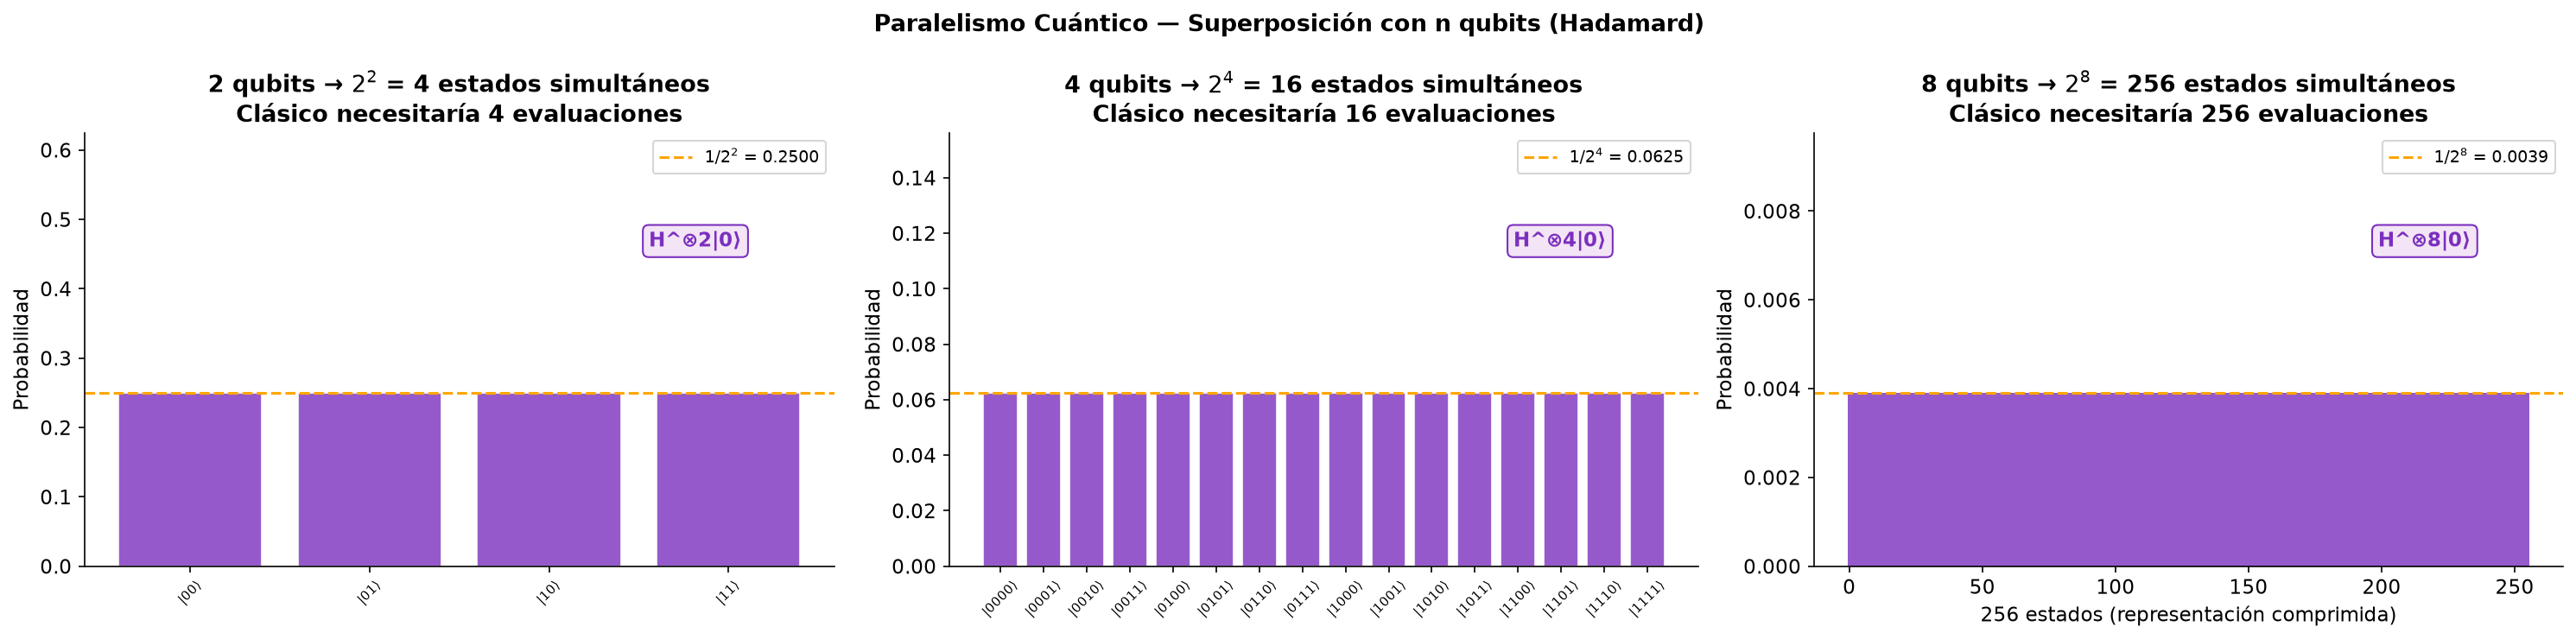
\includegraphics[width=0.95\textwidth]{../POCs/data/output/figures/07_paralelismo_cuantico.png}
\caption{Superposición de $n$ qubits tras aplicar Hadamard a $|0\rangle^{\otimes n}$: el vector de estado tiene $2^n$ amplitudes iguales ($1/2^n$ de probabilidad cada una). Que el espacio de Hilbert crezca exponencialmente no implica que el computador cuántico evalúe $2^n$ casos a la vez: una medición devuelve un único resultado, y la ventaja de algoritmos como Grover o Shor proviene de la interferencia, no del mero paralelismo.}
\label{fig:paralelismo_cuantico}
\end{figure}

\subsection{Patrones transversales}

Los resultados evidencian tres patrones transversales que son coherentes con el estado actual de la teoría y la tecnología cuántica:

\begin{enumerate}
  \item \textbf{La ventaja cuántica requiere alineación dato--feature map}: La ventaja observada en datos nativos es coherente con \cite{huang2021}: el feature map (ZZ u otro) debe estar alineado con el generador; ZZ es el mapa validado empíricamente en este TFM, no un monopolio. En datos reales sin esa alineación, Gradient Boosting y Random Forest mantienen su superioridad.

  \item \textbf{El cuello de botella es la escala}: En todos los casos, la principal limitación práctica del enfoque cuántico no es la calidad del algoritmo sino el coste cuadrático del kernel ($O(n^2)$) y el número de qubits disponibles \citep{haug2023, cerezo2021}. Esta limitación es una función del hardware actual, no del algoritmo en sí.

  \item \textbf{Los resultados negativos son informativos}: Los casos donde el QSVM o el QK-SVR son inferiores a los clásicos en datos reales no son fracasos experimentales, sino resultados metodológicamente valiosos que delimitan el dominio de aplicabilidad. El Caso~8 añade el mismo matiz en one-class: OCSVM-ZZ no sustituye IsolationForest salvo cuando la novedad está alineada con el mapa (aquí \texttt{zz\_phase}), no cuando es geométrica clásica.
\end{enumerate}

\subsection{Implicaciones para la adopción empresarial}

Desde la perspectiva de SKG Tecnología, los resultados sugieren que la integración de algoritmos cuánticos en los sistemas de gestión de movilidad urbana requiere dos condiciones previas: (i) hardware cuántico con mayor número de qubits lógicos y menor tasa de error \citep{preskill2018, cerezo2023}, para operar sobre más features sin reducción dimensional, y (ii) ingeniería de features específica que alinee la representación de los datos con las estructuras geométricas accesibles por los kernels cuánticos \citep{huang2021}. En el corto plazo (horizonte 2--5 años), el valor más realista de la computación cuántica para SKG reside en los algoritmos de optimización combinatoria (QAOA, VQE) para problemas de asignación de recursos, donde la ventaja ya es demostrable a escala moderada con el hardware actual \citep{farhi2014}.

El hilo conductor de los nueve casos de uso es precisamente la demostración de que los algoritmos cuánticos no necesitan reemplazar a los clásicos para ser útiles: basta con que resuelvan de forma más eficaz la parte del problema que es intratable para la computación clásica \citep{biamonte2017}. El Caso~7 lo ilustra de forma paradigmática: aplicar QAOA al conjunto dominante mínimo ---un problema NP-difícil--- y conectarlo con un optimizador clásico COBYLA a través de una interfaz mínima es exactamente el patrón con el que la computación cuántica puede integrarse en entornos productivos reales \citep{farhi2014}. El prototipo de arquitectura híbrida desarrollado en la Sección~\ref{sec:prototipo_hibrido} del Capítulo~\ref{cap:metodologia} formaliza este patrón y define los criterios de activación del módulo cuántico según el tipo de problema.

\subsection{Resultados adicionales y visualización}

El análisis de escalabilidad del caso~1 se sintetiza en la Figura~\ref{fig:escala_clasificacion}: ventaja positiva en $n \in [30, 180]$ \textbf{solo} en el régimen cuántico-nativo (una partición por tamaño). La geometría de kernel se reporta vía los indicadores tabulares del Capítulo~\ref{cap:investigacion_original} ($\Delta A$, $d_F$, $\Delta H$); no se usan heatmaps regenerados a posteriori (las matrices $K$ no se exportaron a artefactos). $\mathcal{Q}>0$ vs.\ un baseline débil no basta como veredicto operativo.

